\chapter{Solutions to Selected Exercises}

\solution{exr:time-compl:2}%{ex:1.1,.1}
 The equation $T(n)=cn^2$ has only one unknown, $c$, to be found
from $T(10) = c\times10^2 = 500$, so $c=500/100 = 5$. Then 
$T(1000)=5\times(1000)^2=5\times10^6$, that is,
the algorithm takes 5 million elementary operations to process 1000 data items.

In fact we do not need to compute $c$. We first compute $T(1000)/T(10)$ which 
equals $10^6c/100c = 10^4$. Thus the answer is $500 \times 10^4$, or 5 million.

%\if 01
%%
\solution{exr:time-compl:7A}%{ex:1.1.2}
As above, the constants \(c_\mathrm{A}\) and \(c_\mathrm{B}\) have to be found
in order to 
work out how many elementary operations 
each algorithm takes with \(n=2^{20}\) and find the fastest algorithm for 
processing \(2^{20}\) data items.
For $n=2^{10}$, $T_\mathrm{A}(2^{10})=c_\mathrm{A}\times 2^{10} \lg(2^{10}) = 10$, 
so $c_\mathrm{A}\times2^{10}\times10 = 10$,
or $c_\mathrm{A}= 1/2^{10} = 2^{-10}$, and $T_\mathrm{B}(2^{10})=c_B  \times(2^{10})^2 = 1$, 
so $c_\mathrm{B}= 2^{-20}$.
Hence,
\[
\begin{array}{rcccllll}
T_\mathrm{A}(2^{20}) & = & 2^{-10} \times 2^{20} \times \lg(2^{20}) 
                                                     & = & 2^{10} \times 20 & < & 2^{15}\\
T_\mathrm{B}(2^{20}) & = & 2^{-20} \times (2^{20})^{2} & = & 2^{20}
\end{array}
\]
and \(T_A(2^{20}) < T_B(2^{20})\), so the algorithm A processes \(2^{20}\) 
data items the fastest.
%%
%\fi

\solution{exm:nest1}%{ex:1.2.1}
The running time is linear because when \(j=m=1\) the assignment statement makes \(m\) 
equal to \(n-1\). Then when \(j=n-1\), the assignment statement makes \(m\) equal to 
\((n-1)^2\). As the inner loop runs once every time \(j=m\), it runs in total only two 
times and does \(n\) operations each loop. The outer loop runs \(n\) times. 
Let $c_\mathrm{i}$ be the constant number of elementary operations in the inner loop, 
and let $c_\mathrm{o}$ be the
number of elementary operations in the outer loop other than the operations in 
the inner loop. 
Then $T(n) = c_\mathrm{o}n + 2c_\mathrm{i}n \in O(n)$.

\solution{exr:aa:bigO:a}%{ex:1.3.1}
We have $10n^3-5n+15 \in O(n^2)$  if and only if (iff) there exist a positive real 
constant $c$ 
and a positive integer $n_0$ such that the inequality \(10n^3-5n+15 \leq cn^2\) 
holds for all $n \ge n_0$ .
Reducing it to \(n -0.5n^{-1} + 1.5n^{-2} \leq 0.1c\) shows 
that for any value of \(c\) this inequality does not hold true for all \(n> k + 1\), 
where $k$ is the
closest integer greater than $0.1c$. Therefore, $10n^3-5n+15 \notin O(n^2)$.

%\if 01
%%
\solution{exr:aa:bigO:b}%{ex:1.3.2}
As above, 
$10n^3-5n+15 \in \Theta(n^3)$ iff there exist positive real constants $c_1$ and $c_2$ 
and a positive integer $n_0$
such that the inequalities
\(c_1n^3 \leq 10n^3-5n+15 \leq c_2n^3\), or what is the same, 
\(c_1 \leq 10-5n^{-2}+15n^{-3} \leq c_2\), hold true
for all $n \ge n_0$ . We know that \(\lim_{n \rightarrow \infty}(10-5n^{-2}+15n^{-3})=10\), 
so there always will be a value  \(n_0 > 3 \) such that 
for \(n>n_0\), \( c_1\leq 10-5n^{-2}+15n^{-3} \leq c_2\) where
\(c_1 \leq 10 - \varepsilon\) and \(c_2 \geq 10 - \varepsilon\) where
$\varepsilon = 5n^{-2}_0 - 15n^{-3}_0 > 0$,
say \(c_1=1\) and \( c_2=20\). Therefore, $10n^3-5n+15 \in \Theta(n^3)$.

Note that Lemma~\ref{l:bigoh:lim}, the Limit Rule, can be used instead. In this case 
\(f(n) = 10n^3-5n+15\); \(g(n)=n^3\), and  \(f(n) \in \Theta(g(n))\) because
\(\lim_{n \rightarrow \infty}\frac{f(n)}{g(n)}=10\). 

%%
%\fi
\solution{exr:aa:bigO:c}%{ex:1.3.3}
As above, $10n^3-5n+15 \in \Omega(n^4)$ iff there exist a positive real constant 
$c$ and a positive integer $n_0$
such that the inequality $10n^3-5n+15 \geq c n^4$ holds for all $n > n_0$. 
We need to show that 
for any value of \(c\) and \(n_0\) this inequality, or what is the same, the reduced one,
\(10n^{-1}-5n^{-3}+15n^{-4}\geq c\), does not hold true for all \(n > n_0\). We know 
\(\lim_{n \rightarrow \infty}(10n^{-1}-5n^{-3}+15n{-4})=0\), 
so no matter which values \(c\) and \(n_0\) are picked, the inequality cannot be true for 
all \(n > n_0\). 
Therefore, $10n^3-5n+15 \notin \Omega(n^4)$.

\if 01
\solution{exr:big:theta}%{ex:1.3.4}
The definition for \(g(n) \in \Theta(f(n))\), namely, that
\(g(n) \in \Theta(f(n))\) iff there exist positive real constants $c_1$ and $c_2$ and a 
positive integer
 $n_0$ such that the inequalities  \(c_1f(n)\leq g(n)\leq c_2f(n)\) hold true for 
all $n\geq n_0$,
contains the definitions for both ``Big Omega" (the left inequality) and 
``Big Oh" (the right inequality).
\fi

%\if 01
%%
\solution{exr:bigoh-order}%{ex:1.3.5}
To show that each function \(f(n)\) in Table~\ref{t:growth} stands in ``Big Oh" relation to the preceding one, $g(n)$,
that is, $f(n) \in O(g(n))$, it is sufficient to use the Limit Rule (Lemma~\ref{l:bigoh:lim}) and 
show that $\lim_{n\rightarrow\infty}f(n) / g(n) = 0$:
\begin{itemize}
\item[] \hspace*{-10mm} $n \in O(n\log{n})$ because 
$n/(n\log n) = (\log n)^{-1}$ and $\lim_{n\rightarrow\infty} (\log n)^{-1} = 0$;
\item[] \hspace*{-10mm} $n\log{n} \in O(n^{1.5})$ because $n\log{n} / n^{1.5} = \log n / n^{0.5}$ 
and any positive power of $n$ grows faster than any 
logarithm (Example~\ref{ex:logs}): \(\lim_{n\rightarrow\infty}\log{n} / n^{0.5} = 0\);
\item[] \hspace*{-10mm} $n^{1.5} \in O(n^2)$ and  $n^2 \in O(n^3)$ because higher powers of  $n$
grow faster than lower powers (Example~\ref{ex:powers}); 
\item[] \hspace*{-10mm} $n^3 \in O(2^n)$ because exponential functions with base greater than 1 
grow faster than any positive power of \(n\) (Example~\ref{ex:expons}):
so \(\lim_{n\rightarrow\infty}n^3/2^n = 0\).
\end{itemize}
%%

\solution{exr:bigoh:features}%{ex:1.3.6}
\noindent{\textbf{Lemma~\ref{l:bigoh:2}}} 
\begin{proof}
It follows from $h(n) \in O(g(n))$ and 
$g(n) \in O(f(n))$ that $h(n) \leq c_1g(n)$ for all $n > n_1$ and
$g(n) \leq c_2f(n)$ for all $n > n_2$ where $c_1$ and $c_2$ are 
positive real constants and
$n_1$ and $n_2$ are positive integers. 
Then $h(n) \leq c_1g(n) \leq c_1 c_2 f (n)$
for $n \geq \max\{n_1,n_2\}$,
so the relationship $h(n) \leq cf(n)$ for all $n \geq n_0$ is also true
for $c = c_1c_2$ and $n_0 = \max\{n_1,n_2\}$. 
Therefore ``Big Oh" is transitive.
\end{proof}

\noindent{\textbf{Lemma~\ref{l:bigoh:3}}} % rule of sums
\begin{proof}
It follows from $g_1(n) \in O(f_1(n))$ and $g_2(n) \in O(f_2(n))$ that 
$g_1(n) \leq c_1f_1(n)$ for all $n > n_1$ and
$g_2(n) \leq c_2f_2(n)$ for all $n > n_2$, respectively, with 
positive real constants  $c_1$ and $c_2$ and positive integers
$n_1$ and $n_2$. Then for all $n \geq \max\{n_1,n_2\}$ 
this is also true: 
\[
g_1(n) + g_2(n) \leq c_1f_1(n)  + c_2f_2(n) \leq \max\{c_1,c_2\}\left(f_1(n)+f_2(n)\right)
\] 
But 
$f_1(n)+f_2(n)\leq 2\max\{f_1(n),f_2(n)\}$, so 
$g_1(n)+g_2(n)\leq c\max\{f_1(n),f_2(n)\}$ where $c = 2\max\{c_1,c_2\}$.
Therefore, $g_1(n)+g_2(n) \in O(\max\{f_1(n),f_2(n)\})$, and  the rule of sums for ``Big Oh" is true.
\end{proof}

%\newpage
\noindent{\textbf{Lemma~\ref{l:bigoh:4}}}  % rule of products
\begin{proof}
It follows from $g_1(n) \in O(f_1(n))$ and $g_2(n) \in O(f_2(n))$ that 
$g_1(n) \leq c_1f_1(n)$ for all $n > n_1$ and
$g_2(n) \leq c_2f_2(n)$ for all $n > n_2$, respectively, with 
positive real constants $c_1$ and $c_2$ and positive integers
$n_1$ and $n_2$. Then for all $n \geq \max\{n_1,n_2\}$ 
this is also true: $g_1(n)g_2(n) \leq %c_1f_1(n)c_2f_2(n)$, or $g_1(n)g_2(n) \leq 
cf_1(n)f_2(n)$ where $c=c_1c_2$. 
Therefore the rule of products for ``Big Oh" is true.
\end{proof}

%%
%\fi
\solution{exr:bigomega:sums}%{ex:1.3.7}
The rule of sums for ``Big Omega" and ``Big Theta" is similar to that
for ``Big Oh", namely,
\begin{itemize}
\item[] \hspace*{-10mm} If $g_1\in\Omega(f_1)$ and $g_2\in\Omega(f_2)$, then 
$g_1 + g_2\in\Omega(\max\{f_1,f_2\})$, and
\item[] \hspace*{-10mm} If $g_1\in\Theta(f_1)$ and $g_2\in\Theta(f_2)$, then 
$g_1 + g_2\in\Theta(\max\{f_1,f_2\})$. 
\end{itemize} 

\solution{exr:bigomega:lem}%{ex:1.3.8}
The Lemmas and proofs are similar to the ``Big Oh" ones, 
except the inequalities are ``greater than" instead of ``less than".

\noindent\textbf{Lemma~\ref{l:bigoh:1} (Scaling).} For all constants $c > 0$, $cf\in\Omega(f)$,
in particular, $f\in\Omega(f)$.
\begin{proof}
The relationship \(cf(n) \geq cf(n)\) holds for all \(n > 0\). 
Thus, constant factors are ignored.
\end{proof}
\noindent\textbf{Lemma~\ref{l:bigoh:2} (Transitivity).}
If $h\in\Omega(g)$ and $g\in\Omega(f)$, then $h\in\Omega(f)$.
\begin{proof}
It follows from $h(n) \in \Omega(g(n))$ and 
$g(n) \in \Omega(f(n))$ that $h(n) \geq c_1g(n)$ for all $n > n_1$ and
$g(n) \geq c_2f(n)$ for all $n > n_2$ where $c_1$ and $c_2$ are 
positive real constants and
$n_1$ and $n_2$ are positive integers. 
Then $h(n) \geq c_1g(n) \geq c_1 c_2 f (n)$,
or $h(n) \geq cf(n)$ is also true
for $c = c_1c_2$ and all $n \geq n_0 = \max\{n_1,n_2\}$. 
Therefore Big Omega is transitive.
\end{proof}
\noindent\textbf{Lemma~\ref{l:bigoh:3} (Rule of sums).}
If $g_1\in\Omega(f_1)$ and $g_2\in\Omega(f_2)$, then 
$g_1 + g_2\in\Omega(\max\{f_1,f_2\})$.
\begin{proof}
It follows from $g_1(n) \in \Omega(f_1(n))$ and $g_2(n) \in \Omega(f_2(n))$ that 
$g_1(n) \geq c_1f_1(n)$ for all $n > n_1$ and
$g_2(n) \geq c_2f_2(n)$ for all $n > n_2$, respectively, with 
positive real constants  $c_1$ and $c_2$ and positive integers
$n_1$ and $n_2$. Then for all $n \geq \max\{n_1,n_2\}$ 
this is also true: 
\[
g_1(n) + g_2(n) \geq c_1f_1(n)  + c_2f_2(n) \geq \min\{c_1,c_2\}\left(f_1(n)+f_2(n)\right)
\] 
But 
$f_1(n)+f_2(n)\geq \max\{f_1(n),f_2(n)\}$, so 
$g_1(n)+g_2(n)\geq c\max\{f_1(n),f_2(n)\}$ where $c = \min\{c_1,c_2\}$.
Therefore, $g_1(n)+g_2(n) \in \Omega(\max\{f_1(n),f_2(n)\})$, and  the rule of sums 
for ``Big Omega" is true.
\end{proof}
\noindent{\textbf{Lemma~\ref{l:bigoh:4}}}  (\textbf{Rule of products}).
Similar to the above lemmas.

\if 01
\begin{proof}
It follows from $g_1(n) \in \Omega(f_1(n))$ and $g_2(n) \in \Omega(f_2(n))$ that 
$g_1(n) \geq c_1f_1(n)$ for all $n > n_1$ and
$g_2(n) \geq c_2f_2(n)$ for all $n > n_2$, respectively, with 
positive real constants $c_1$ and $c_2$ and positive integers
$n_1$ and $n_2$. Then for all $n \geq \max\{n_1,n_2\}$ 
this is also true: $g_1(n)g_2(n) \geq %c_1f_1(n)c_2f_2(n)$, or $g_1(n)g_2(n) \geq 
cf_1(n)f_2(n)$ where $c=c_1c_2$. 
Therefore the rule of products for ``Big Omega" is true.
\end{proof}
\fi

%\newpage 
\solution{exr:aa:data-size}%{ex:1.4.2}
You can make \(n\) the subject of the equation for all \(f(n)\) except for 
\(n\lg{n}\). 
To work out \(n\lg{n}\), simply guess \(n\) until you find the correct 
value for 1 millennium.

\begin{center}
\begin{tabular}{|c|c|c|}
\hline
& \multicolumn{2}{c|}{\textbf{Length of time to run an algorithm}} \\
\cline{2-3}
\(f(n)\)& 1 century & 1 millennium \\
\hline
\(n\)& $5.26 \times 10^9$ & \(5.26 \times 10^9 \)\\
\hline
\(n\lg{n}\)&$6.72 \times 10^7$ & \( 5.99 \times 10^8\) \\
\hline
\(n^{1.5}\)&$1.40 \times 10^6$ & \(6.51 \cdot 10^6\) \\
\hline
\(n^2\)& 72 522& 229 334\\
\hline
\(n^3\)& 3 746 & 8 071\\
\hline
\(2^n\)& 35 & 39\\
\hline
\end{tabular}
\end{center}

%\if 01
\solution{exr:aa:time-cmplx}%{ex:1.4.1}
\begin{center}
\begin{tabular}{|c|c|cccc|c|}
\hline
\multicolumn{2}{|c|}{\textbf{Time complexity}} &\multicolumn{4}{|c|}{\textbf{Input size} \(n\)}& \textbf{Time} \(T(n)\) \\
\cline{1-6} 
\textit{Function}& \textit{Notation}& \textit{10}& \textit{30}& \textit{100}& \textit{1000}& \\
\hline
``\(\log{\log{n}}\)"& \(\lg{\lg{n}}\)& 1& 1.23& 1.42& 1.68& \(\lg{\lg{n}} / \lg{\lg{10}}\) \\
\hline 
``\(n^2\log{n}\)"&\(n^2\lg{n}\)& 1& 13.29& 200& 30000& \( n^2\lg{n} / 100\lg{10} \)\\
\hline
\end{tabular}
\end{center}
%%
%\fi

\solution{exr:rec-low-bound}%{ex:1.5.1}
The recurrence $T(n) = T(n-1) + n$; $T(0)=0$, in Example~\ref{exm:recur:a} implies that 
$T(n) \geq 0$ for $n\geq 0$, so $T(n) \geq n$ 
for all $n > 0$. Therefore, \(T(n)\in\Omega(n)\) for general \(n\). Similarly,
$T(n) \geq 0 $ for all $n\geq 0$, so $T(n) \geq n$ for all $n > 0$ and 
therefore, $T(n)\in\Omega(n)$ in Examples~\ref{exm:recur:c} and~\ref{exm:recur:d}.

Conversely, in Example~\ref{exm:recur:b} $T(n)\notin\Omega(n)$ because 
$T(n) \leq \lceil\lg n\rceil < \lg(n+1)$ for all $n\geq 2$, and the 
logarithmic function grows slower than $n$ (Example~\ref{ex:logs}).

\solution{exr:rec-mergesort} %1.5.2
The base case holds for $n=2$: $T(2)=T(1)+T(1)+2 = 2 < 3 = 2\lg2 + 2 -1$.
By the inductive hypothesis, $T(m) \leq m\lg m + m - 1 = m(\lg m + 1) - 1$ for all $m < n$.
For an even $n$, $\lceil \frac{n}{2} \rceil =  \lfloor \frac{n}{2}  \rfloor = \frac{n}{2}$,
so
\[
\begin{array}{lll}
T(n) & \leq & 2\left(\frac{n}{2}\left(\lg\left(\frac{n}{2}\right) + 1\right) - 1\right) = n\lg n - 2 \leq n\lg n + n - 1;\;\;n\geq 4
\end{array}
\]
For an odd $n$, $\lceil \frac{n}{2} \rceil = \frac{n+1}{2}$; 
$\lfloor \frac{n}{2}  \rfloor = \frac{n-1}{2}$, and $\lg(n-1) < \lg(n+1) < \lg n + 1$, so
\[
\begin{array}{lll}
T(n)& \leq & \frac{n+1}{2}\lg\left(\frac{n+1}{2}\right) + \frac{n-1}{2}\lg\left( \frac{n-1}{2}\right) + \frac{n+1}{2} + \frac{n-1}{2} - 2 \\ \\
& \leq & \frac{n+1}{2}\lg(n+1) + \frac{n-1}{2}\lg(n-1) - 2 \\ \\
& \leq  & \frac{n+1}{2} \left(\lg n + 1\right) + \frac{n-1}{2} \left(\lg n + 1 \right) - 1 = n\lg n + n - 1; \; \; n \geq 3
\end{array}
\]
Therefore, for all $n \geq 2$, $T(n) \leq n\lg n + n - 1$.

\solution{exr:recur:cn}%{ex:1.5.3}
Substituting \(n=k^m\) into the recurrence 
\(T(n) =kT\left(\frac{n}{k}\right)+cn\); \(T(1)=0\) gives
\( T(k^m) = kT(k^{m-1})+ck^m\); \(T(k^0)=0\). Telescoping the latter recurrence yields:
\begin{eqnarray*}
T(k^m) &=& kT(k^{m-1}) + ck^m \\
             &=& k\left(kT(k^{m-2})+ ck^{m-1}\right) + ck^m\\ 
             &=&k^2T(k^{m-2}) + 2ck^m \\
T(k^m) &=& k^2\left(kT(k^{m-3})+ck^{m-2}\right) + 2ck^m\\
             &=& k^3T(k^{m-3}) + 3ck^m\\
             &.\ldots& \\
T(k^m) &=& k^mT(1) + cmk^m \\
              &=& cmk^m 
\end{eqnarray*}
or, what is the same, $T(n) = cn\log_k{n}$.
Therefore, \(T(n) \in O(n\log{n})\).

%\newpage
\solution{exr:recur:ckn}%{ex:1.5.4}
Just as in the previous solution, substituting \(n=k^m\) into the recurrence 
\(T(n) =kT(\frac{n}{k})+ckn\); \(T(1)=0\),
produces \(T(k^m) = kT(k^{m-1})+ck^{m+1}\); \(T(1)=0\).
Telescoping the latter recurrence gives:
\begin{eqnarray*}
T(k^m) &=& kT(k^{m-1}) + ck^{m+1} \\
             &=& k\left(kT(k^{m-2})+ ck^m\right) + ck^{m+1} \\
             &=&k^2T(k^{m-2}) + 2ck^{m+1} \\
T(k^m) &=& k^2\left(kT(k^{m-3})+ck^{m-1}\right) + 2ck^{m+1}\\
             &=& k^3T(k^{m-3}) + 3ck^{m+1}\\
             &.\ldots& \\
T(k^m) &=& k^mT(1) + cmk^{m+1} \\
              &=& cmk^{m+1} = ckmk^m
\end{eqnarray*}
or, what is the same, \(T(n) = ckn\log_k{n}\).
Therefore, \(T(n) \in O(n\log{n})\).

\solution{exr:alg-compar:1}%{ex:1.7.1}
Because \(n \in O(n\log{n})\), in ``Big-Oh" sense the linear algorithm \textbf{B} 
has better performance than the ``\(n\log{n}\)" algorithm \textbf{A}. But for 
small enough \(n\), the latter algorithm is faster,
e.g. $T_\mathbf{A}(10) = 50$ and $T_\mathbf{B}(10)=400$ elementary operations. The cutoff point is when 
\(T_{\textbf{A}}(n) = T_{\textbf{B}}(n)\), that is:
\(
5n\log_{10}n = 40n,\textrm{  or  }\log_{10}n = 8,\textrm{  or  }n = 10^8
\).
Therefore, even though the algorithm \textbf{B} is faster in ``Big Oh" sense, 
this only occurs when more than 100 million data items have to be processed. 

\solution{exr:alg-compar:2}%{ex:1.7.2}
In ``Big-Oh" sense, the average-case time complexity of the 
linear algorithm \textbf{A} is larger than of the ``$\sqrt{n}$" algorithm \textbf{B}. 
But for a database of the given size, $T_{\mathbf{A}}(10^9) = 10^6$ and 
$T_{\mathbf{B}}(10^9) = 1.58 \times 10^7$ elementary operations. So in this case the 
algorithm \textbf{A} is, in the average,
over ten times faster than the algorithm \textbf{B}. Because we can tolerate the risk of an
occasional long running time that might occur more likely with the more complex 
algorithm, the algorithm \textbf{A} should be used.

\solution{exr:selectionsort}
Regardless of the initial ordering of the list, selection sort searches at each iteration $i$ through the entire unsorted part
of the size $n-i$ and makes $n-i-1$ comparisons to find the minimum element, so in total, 
\(\sum_{i=1}^{n-1}{i}= \frac{n(n-1)}{2} \in \Theta(n^2)\) comparisons in the worst, average, and best case.
The maximum number of data moves is \(n\), because each iteration moves at most one element into its 
correct position, and their average number is \(\frac{n}{2}\). 
Thus, both the maximum and the average individual time complexity in selection 
sort is $\Theta(n)$ for data moves and \(\Theta(n^2)\) for comparisons.

\if 01
\solution{exr:isort:sorted:already}
The running time of insertion sort is \(O(n)\) as the inner while loop will never run leaving only \(n-1\) iterations of the outer loop.
This is far faster than the worst case running time of \(O(n^2)\).
Bubble sort is also \(O(n)\), as no swaps will happen so the inner loop will run once doing \(n-1 \in O(n)\) comparisons. Again, it is far faster than the worse case running time of \(O(n^2)\). 
Selection sort has been shown to be \(O(n^2)\) for any array sorting, so both for a sorted array and in the worst case.
\fi

\if 01
\solution{exr:rec-mergesort}
The result is clearly true for $n=1$. Suppose that $n > 1$, and that
 $T(k) \leq k\lg k + k - 1$ holds for all $k < n$.

Using the recurrence and inductive hypothesis we have (for $n$ even)
\begin{align*}
T(n)  &= T(\lceil n/2\rceil) + T(\lfloor n/2 \rfloor) + n \\
& \leq 2 n/2 \lg n/2 + 2 (n/2 - 1) + n \\
& = n (\lg n - 1) + 2n - 2 \\
& = n \lg n + n - 2. 
\end{align*}

For odd $n$ we have similarly (with considerably more algebraic simplification)
\begin{align*}
T(n)  &= T(\lceil n/2\rceil) + T(\lfloor n/2 \rfloor) + n \\
& \leq \frac{n+1}{2} \lg \frac{n+1}{2} + \frac{n+1}{2} - 1 + \frac{n-1}{2} \lg \frac{n-1}{2} + 
\frac{n-1}{2} - 1 + n \\
& = \frac{n+1}{2} \lg (n+1) + \frac{n-1}{2} \lg (n-1) + n - 2 \\
& = n \lg n + n + \left[\frac{n}{2} \lg (1 - n^{-2}) + \frac{1}{2} \lg (1 + \frac{2}{n-1}) - 2\right]
\\
& :=  n \lg n + n - 1 + f(n). 
\end{align*}

The function $f(x) = \left[\frac{x}{2} \lg (1 - x^{-2}) + \frac{1}{2} \lg (1 + \frac{2}{x-1}) - 1\right]$ has derivative (after a little algebraic simplification) equal to 
$\frac{1}{2} \lg (1 - x^{-2})$ which is negative for $x>0$. Thus the maximum value of $f(n)$ 
for $n>1$ occurs when $n=2$, and since its value is negative, we have $f(n) <0$ for 
$n\geq 2$.

Thus the inductive step holds in each case, and so by induction the result is true.
\fi

%\newpage
\solution{exr:isort:inverse}%{ex:2.1.1}
Adding up the columns in the next table gives, in total, 90 comparisons 
plus data moves. 
\begin{center}
\begin{tabular}{|c|c|c|c|c|c|c|c|c|c|c|c|c|}
\hline
\(i\)& \(C_i\)& \(M_i\) &\multicolumn{10}{|c|}{\textbf{Data to sort}} \\
\hline
\multicolumn{3}{|c|}{}& 91& \textbf{70}& 65& 50& 31& 25& 20& 15& 8& 2 \\
\hline
1& 1& 1& \underline{70} & 91& \textbf{65}& 50& 31& 25& 20& 15& 8& 2 \\
\hline
2& 2& 2& \underline{65} & 70& 91& \textbf{50}& 31& 25& 20& 15& 8& 2 \\
\hline
3& 3& 3& \underline{50} & 65& 70& 91& \textbf{31}& 25& 20& 15& 8& 2 \\
\hline
4& 4& 4& \underline{31} & 50& 65& 70& 91& \textbf{25}& 20& 15& 8& 2 \\
\hline
5& 5& 5& \underline{25} & 30& 50& 65& 70& 91& \textbf{20}& 15& 8& 2 \\
\hline
6& 6& 6& \underline{20} & 25& 30& 50& 65& 70& 91& \textbf{15}& 8& 2 \\
\hline
7& 7& 7& \underline{15} & 20& 25& 30& 50& 65& 70& 91& \textbf{8}& 2 \\
\hline
8& 8& 8& \underline{8} & 15& 20& 25& 30& 50& 65& 70& 91& \textbf{2} \\
\hline
9& 9& 9& \underline{2} & 8& 15& 20& 25& 30& 50& 65& 70& 91 \\
\hline
\end{tabular}
\end{center}

\solution{exr:isort2}%{ex:2.1.2}
The inductive hypothesis is that each inner-loop iteration $i = 1,\ldots,n-1$ of insertion sort increases by one
the size of the already sorted part $a[0],\ldots, a[i-1])$ of size $i$
in the list under consideration, while keeping it sorted.
The base case for the math induction is for $i=0$ when the sorted part $(a[0])$ of size $1$ is sorted by definition. 
%%%%%%%%%%%%%%%%%%%%
At iteration $i$, an element  $temp$ from the
unsorted part of the list is inserted into the already sorted part
between the elements $a[j-1]$ and $a[j]$ such that $a[j-1]\leq temp < a[j]$. 
Either the left-hand  or right-hand inequality may be absent if $j=0$ or $j=i$, respectively. 
The obtained new part of size $i+1$ is sorted because
all the previous elements smaller than or equal to \(temp\) are before it
and stay sorted, 
and all elements greater than \(temp\) are after it and also stay sorted. 
So because the iterations terminate when $i > n-1$, 
insertion sort is correct.

Moreover, duplicates will be lumped together and
their relative order in the initial unsorted array will not change, so insertion sort
is {\em stable}.
%\newpage

\solution{exr:isort:max}%{ex:2.1.3}
Insertion sort runs the slowest on the totally reverse ordered list that
has the maximum number of inversions: \( \binom{n}{2} = \frac{n(n-1)}{2}\in\Theta(n^2)\).
The worst-case time complexity of insertion sort is \(\Theta(n^2)\) because each 
swap removes only one inversion.

%%
\solution{exr:inversions}%{ex:2.1.4}
Obviously, sorting of elements that precede $a[i]$ (i.e. with positions less than $i$) does not change their inversions with \(a[i]\). 
So the number $\nu$ of inversions between \(a[i]\) and the preceding elements
is equal to the total number of elements greater than \(a[i]\) among the elements $a[0],\ldots,a[i-1]$. Just before 
the iteration $i$ places the element \(a[i]\) into its correct position, the preceding sorted part will have the $\nu$ elements;
$0\leq\nu\leq i$, being greater than \(a[i]\) and ordered
immediately before $a[i]$ at the positions $i-1,\ldots,i-\nu$. During execution of insertion sort on an array, every element 
of the array that is greater 
than \(a[i]\) must be moved up once. Thus the 
total number of data moves to insert \(a[i]\) is equal to the total number \(\nu\) of inversions with respect to the preceding elements 
in the initial array.

%\if 01
\solution{exr:num:inversions}%{ex:2.1.5} 
The out-of-order elements \(a[i]\) and \(a[i+gap]\) are not equal one to another, so $a[i] > a[i+gap]$.
The elements at positions less than \(i\) or greater than \(i+gap\) do not change 
their inversions with respect to either \(a[i]\) or \(a[i+gap]\) after the latter are swapped. 
The swap adds no new inversions with the elements, $a[k]$; $i < k < i+gap$,   between these positions
because all the already ordered pairs such that $a[i] < a[k]$ and $a[k] < a[i+gap]$  
remain ordered after this swap. Since no inversions are added but one inversion is removed 
by placing \(a[i]\) and \(a[i+gap]\) in order, the minimum number of the inversions removed is 1. 

The maximum number of the inversions is removed if for every pair of positions (\(i,k\)) or (\(k,i+gap\)) where \(i < k < i+gap\) there 
was an inversion before, but no inversion after the swap. There are \(2\times(gap-1)\) such pairs, so the maximum
number of the inversions removed is \(2\times gap-1\). 
Thus, swapping the out-of-order elements \(a[i]\) and \(a[i+gap]\) of a list \(a\) removes at least \(1\) and at most \(2\times gap-1\)
inversions.

%%
%\fi
\solution{exr:bubblesort}%{ex:2.1.6}
The while loop runs until there are no data swaps in the inner for-loop, so the while loop 
stops just after the list is sorted. Each swap of elements $a[i]$ and $a[i-1]$ in the inner for-loop 
removes exactly one inversion, does not affect their inversions with the preceding
or subsequent elements in the list, and obviously does not create any new inversion. Because the average
number of inversions in a list is $\frac{1}{2}\binom{n}{2} = \frac{n(n-1)}{4}\in O(n^2)$, the 
average time complexity of bubble sort is $O(n^2)$.

%\newpage
\solution{exr:comparedata}%{ex:2.1.9}
\begin{center}\footnotesize
\begin{tabular}{|c|c|c|c|c|c|c|c|c|c|c|c|c|c|}
\hline
\(h\)& \(i\)& \(C_i\)& \(M_i\) &\multicolumn{10}{|c|}{\textbf{Data to sort}} \\
\hline
5& \multicolumn{3}{|c|}{}& 91& 70& 65& 50& 31& 25& 20& 15& 8& 2 \\
\cline{2-14}
& 5& 1& 1& \textbf{25}& & & & & \textbf{91}& & & & \\
\cline{2-14}
& 6& 1& 1& & \textbf{20}& & & & & \textbf{70}& & & \\
\cline{2-14}
& 7& 1& 1& & & \textbf{15}& & & & & \textbf{65}& & \\
\cline{2-14}
& 8& 1& 1& & & & \textbf{8}& & & & & \textbf{50}& \\
\cline{2-14}
& 9& 1& 1& & & & & \textbf{2}& & & & & \textbf{31} \\
\hline
2& \multicolumn{3}{|c|}{}& 25& 20& 15& 8& 2& 91& 70& 65& 50& 31 \\
\cline{2-14}
& 2& 1& 1& \textbf{15}& & \textbf{25}& & & & & & & \\
\cline{2-14}
& 3& 1& 1& & \textbf{8}& & \textbf{20}& & & & & & \\
\cline{2-14}
& 4& 2& 2& \textbf{2}& & \textbf{15}& & \textbf{25}& & & & & \\
\cline{2-14}
& 5& 1& 0& & & & 20& & 91& & & & \\
\cline{2-14}
& 6& 1& 0& & & & & 25& & 70& & & \\
\cline{2-14}
& 7& 2& 1& & & & 20& & \textbf{65}& & \textbf{91}& & \\
\cline{2-14}
& 8& 2& 1& & & & & 25& & \textbf{50}& & \textbf{70}& \\
\cline{2-14}
& 9& 3& 2& & & & 20& & \textbf{31}& & \textbf{65}& & \textbf{91} \\
\hline
1& \multicolumn{3}{|c|}{}& 2& 8& 15& 20& 25& 31& 50& 65& 70& 91 \\
\cline{2-14}
& 1& 1& 0& 2& 8& & & & & & & & \\
\cline{2-14}
& 2& 1& 0& & 8& 15& & & & & & & \\
\cline{2-14}
& 3& 1& 0& & & 15& 20& & & & & & \\
\cline{2-14}
& 4& 1& 0& & & & 20& 25& & & & & \\
\cline{2-14}
& 5& 1& 0& & & & & 25& 31& & & & \\
\cline{2-14}
& 6& 1& 0& & & & & & 31& 50& & & \\
\cline{2-14}
& 7& 1& 0& & & & & & & 50& 65& & \\
\cline{2-14}
& 8& 1& 0& & & & & & & & 65& 70& \\
\cline{2-14}
& 9& 1& 0& & & & & & & & & 70& 91\\
\hline
\end{tabular}
\end{center}

By adding up the columns, we get a total of 40 comparisons plus data moves. 
This is less than half that of insertion sort's 90, 
so even with a low \(n\) value, Shellsort is better than insertion sort.

\solution{exr:insertion+merge}
Insertion sort runs in \(\Theta(n^2)\) in the average and worst case, so
the total time for this algorithm is:
\[
T(n) =k c \left( \frac{n}{k} \right)^2 + c(k-1)n = c \frac{n^2}{k} + c(k-1)n  
= cn \left( \frac{n}{k} + (k-1) \right)  
\]
Assuming the constant $n$ and the variable $k$, 
\(T(n)\) is minimal for the same value of \(k\) as the function 
\( f_n(k)=\frac{n}{k} + k-1 \). Because \(1 \leq k \leq n\), at the boundaries
\(f_n(1) = n\) and \(f_n(n) = n\), and the function is not equal to \(n\) at every 
other \(k\), at least one local optimum exists in the interval
between \(k=1\) and \(k=n\). For this optimum, the  
first derivative by \(k\) equals to 0:
\(\frac{df_n(k)}{dk} = -\frac{n}{k^2} + 1 \), so \(\frac{n}{k^2} =1 \), or \(k= \sqrt{n} \).
Since \(f_n(\sqrt{n}) = 2\sqrt{n}-1 < n\), it is a local minimum.
Thus, when \(k = \sqrt{n}\), \(T(n) = cn(2\sqrt{n} -1)\) is minimal, too.

It is not as fast as mergesort's \(\Theta(n\log{n})\) but quicker 
than insertion sort's \(\Theta(n^2)\).

\if 01
\solution{exr:qsort:pivot-choice}%{ex:2.3.1}
In the probabilstic sense, chances of running quicksort in quadratic time
are the same for both the dynamic and static passive strategy because the 
probability to meet and select at each step either the maximum or the minimum 
element in each sublist of the size of $k$ remains the same, \(\frac{2}{k}\), in both 
the cases. Under such a selection, at each recurse one out of two sublists is 
always empty, and 
the size of the other sublist decreases by one. Hence, 
the total probability of always selecting the maximum or the minimum is 
the product of the individual probabilities from \(k=n\) to \(k=2\):
\[
\prod\limits_{i=2}^n\frac{2}{i} = \frac{2^{n-1}}{n!} \approx \frac {2^{n-1}e^{n}}{n^{n}\sqrt{2\pi n}}
= \left(\frac{2e}{n}\right)^n \frac{1}{2\sqrt{2\pi n}}
\]
by Stirling's approximation of $n!$. For large $n$, this probability is negligibly small.
But the dynamic strategy stands much better against a malicious adversary.
\fi

%\newpage
\solution{exr:qs-example}%{ex:2.3.2}
Partitioning of a 5-element list after choosing the pivot $p=15$ 
(the bold element is the pivot; elements in italics are those pointed 
to by the pointers $L$ and $R$).

\begin{center}
\begin{tabular}{|c|c|c|c|c|c|}
\hline
\multicolumn{5}{|c|}{\textbf{Data to sort}}& {\textbf{Description}}\\ \hline
20& 8& 2& 25& 15&  Initial array \\ \hline
\textbf{15}& 8& 2& 25& 20& move pivot to head\\ \hline
\textbf{15}& 8& \textit{\large 2}& 25& 20& stop $R$\\ \hline
\textbf{15}& 8& \textit{\large 2}& 25& 20& stop $L$ (as $L=R$)\\ \hline
2 & 8& \textit{15}& 25& 20& swap element $L$ with pivot\\ \hline
\end{tabular}
\end{center}


\if 01
\solution{exr:qs-bad:partition}%{ex:2.3.3}
Partitioning of a 7-element array with \(l=0\), \(m=3\), and \(r=6\). The pivot
\(p=8\) is chosen as the median of \(a[0]=25\), \(a[3]=8\), and \(a[6]=2\).

\begin{center}
\begin{tabular}{|c|c|c|c|c|c|c|c|c|c|}
\hline
\multicolumn{7}{|c|}{\textbf{Data to sort}}& \multicolumn{3}{|c|}{\textbf{Description}}\\
\hline
0& 1& 2& 3& 4& 5& 6& \multicolumn{3}{|l|}{ \(\leftarrow\)Indices} \\
\hline
25& 8& 8& 8& 8& 8& 2& \multicolumn{3}{|c|}{Initial array} \\
\hline
2& 8& 8& 8& 8& 8& 25& \multicolumn{3}{|c|}{median-of-three sort (\( a[l],a[m],a[r] \))} \\
\hline
2& 8& 8& 8& 8& \textbf{8} & 25& \multicolumn{3}{|c|}{ \textbf{swap}(\( p=a[m],a[r-1] \))} \\
\hline
2& 8& 8& 8& 8& \textbf{8} & 25& \(i\)& \(j\)& Condition \\
\hline
& 8& & & 8& \textbf{8}& & 1& 4& \(a[i] \leq p;\; i \leftarrow i+1;\; p \leq a[j]\) \\
\hline
& & 8& & 8& \textbf{8}& & 2& 4& \(a[i] \leq p;\; i \leftarrow i+1;\; p \leq a[j]\) \\
\hline
& & & 8& 8& \textbf{8}& & 3& 4& \(a[i] \leq p;\; i \leftarrow i+1;\; p \leq a[j]\) \\
\hline
& & & & 8& \textbf{8}& & 4& 4& \(a[i] \leq p;\; i \leftarrow i+1;\; p \leq a[j]\) \\
\hline
& & & & 8& \textbf{8}& & 5& 4& \(a[i] \leq p;\; i \leftarrow i+1;\; p \leq a[j]\) \\
\hline
& & & & 8& \textbf{8}& 25& 6& 4& \(a[i] > p;\; p \leq a[j];\; j\leftarrow j-1\) \\
\hline
& & & 8& & \textbf{8}& 25& 6& 3& \(a[i] > p;\; p \leq a[j];\; j\leftarrow j-1\) \\
\hline
& & 8& & & \textbf{8}& 25& 6& 2& \(a[i] > p;\; p \leq a[j];\; j\leftarrow j-1\) \\
\hline
& 8& & & & \textbf{8}& 25& 6& 1& \(a[i] > p;\; p \leq a[j];\; j\leftarrow j-1\) \\
\hline
2& & & & & \textbf{8}& 25& 6& 0& \(a[i] > p;\; p > a[j]\) \\
\hline
& & & & & \textbf{8}& & 6& 0& \(i >j;\;\)\textbf{break} \\
\hline
2& 8& 8& 8& 8& 25& \textbf{8}& \multicolumn{3}{|c|}{swap(\(a[i],p=a[r-1]\))} \\
\hline
\end{tabular}
\end{center}
Because in this case the pointers are advanced also when the pivot is equal to 
the current element, the pointer
\(i\) does not stop before the pivot and 
reaches instead a next element those value AND index are greater than 
for the pivot. The pointer \(j\) stops when reaching the very first
element being less than the pivot. This means the subsequent swap of the pivot and 
\(a[i]\) 
no longer yields a sorted list. 
\fi

\if 01
\solution{exr:quicksort:sorted:already}%{ex:2.3.4}
It depends on how the pivot is chosen. Let us consider 
the median of three and the fixed pivot at the start, middle, or random
position. The median of three and the pivot at the middle position
run in \(O(n\log{n})\) time because always the best pivot is selected
at each step. The random selection will be also \(O(n\log n)\) because
of the very low probability of the quadratic behaviour due to selecting
the min or max element at each step. 
The fixed pivot at the start will run in \(O(n^2)\) time, as it choose 
at each step the 
worst pivot (i.e. the minimum element). 
\fi

\solution{exr:insert:heap}%{ex:2.4.1}
\begin{center}
\begin{tabular}{|l|c|c|c|c|c|c|c|c|c|c|c|c|}
\hline
\textbf{Position}& 1& 2& 3& 4& 5& 6& 7& 8& 9& 10& 11& 12 \\
\hline
\textbf{Index}& 0& 1& 2& 3& 4& 5& 6& 7& 8& 9& 10& 11 \\
\hline
Array at step 1& 91& 75& 70& 31& 65& 50& 25& 20& 15& 2& 8& \textbf{85} \\
\hline
Array at step 2& 91& 75& 70& 31& 65& \textbf{85}& 25& 20& 15& 2& 8& 50 \\
\hline
Array at step 3& 91& 75& \textbf{85}& 31& 65& 70& 25& 20& 15& 2& 8& 50 \\
\hline
\end{tabular}
\end{center}

\if 01
%%%
\solution{ex:min-heap}%{ex:2.4.2}
There is no unique solution. For instance,
building the minimum heap by reversing the order the array keys in Figure 2.8 
and restoring the heap order gives the 
following example:
\begin{center}
\begin{tabular}{|c|c|c|c|c|c|c|c|c|c|c|}
\hline
Position& 1& 2& 3& 4& 5& 6& 7& 8& 9& 10 \\
\hline
Key& 2& 15& 8& 25& 50& 20& 31& 70& 65& 91 \\
\hline
\end{tabular}
\end{center}
%%
\fi

\solution{exr:delete:heap}%{ex:2.4.3}
Restoring the heap after deleting the maximum element:
\begin{center}{\footnotesize
\begin{tabular}{|l|c|c|c|c|c|c|c|c|}
\hline
\textbf{Position}& 1& 2& 3& 4& 5& 6& 7& 8 \\
\hline
\textbf{Index}& 0& 1& 2& 3& 4& 5& 6& 7 \\
\hline
Step 1& \textbf{15}& 65 & 50& 31& 8& 2& 25& 20 \\
\hline
Step 2& \textbf{65}& \textit{15}& 50& 31& 8& 2& 25& 20 \\
\hline
Step 3& 65& \textbf{31}& 50& \textit{15}& 8& 2& 25& 20 \\
\hline
Step 4& 65& 31& 50& \textbf{20}& 8& 2& 25& \textit{15} \\
\hline
\end{tabular}
}
\end{center}

%\if 01
\solution{exr:heap:build}%{ex:2.4.4}
\begin{center}
{\footnotesize
\begin{tabular}{|l|c|c|c|c|c|c|c|c|c|}
\hline
\textbf{Position}& 1& 2& 3& 4& 5& 6& 7& 8& 9 \\
\textbf{Index}& 0& 1& 2& 3& 4& 5& 6& 7& 8 \\
\hline
Initial array& 10& 20& 30& 40& 50& 60& 70& 80& 90 \\
\hline
$i=3$& 10& 20& 30& \textbf{90} & 50& 60& 70& 80& \textit{40} \\
$i=2$& 10& 20& \textbf{ 70}& 90& 50& 60& \textit{30}& 80& 40 \\
$i=1$& 10& \textbf{90}& 70& \textit{20}& 50& 60& 30& 80& 40 \\
     & 10& 90& 70& \textbf{ 80}& 50& 60& 30& \textit{20}& 40 \\
$i=0$& \textbf{ 90}& \textit{10}& 70& 80& 50& 60& 30& 20& 40 \\
     & 90& \textbf{80}& 70& \textit{10}& 50& 60& 30& 20& 40 \\
     & 90& 80& 70& \textbf{40}& 50& 60& 30& 20& \textit{10} \\
\hline
Max heap& 90& 80& 70& 40& 50& 60& 30& 20& 10 \\
\hline
\end{tabular}
}
\end{center}
%
%\fi

%\newpage
\solution{exr:hsort:apply}%{ex:2.4.5}
\begin{center}
{\footnotesize
\begin{tabular}{|l|c|c|c|c|c|c|c|c|c|c|}
\hline
\textbf{Position}& 1& 2& 3& 4& 5& 6& 7& 8& 9& 10 \\
\textbf{Index}& 0& 1& 2& 3& 4& 5& 6& 7& 8& 9 \\
\hline
Initial array& 2& 8& 15& 20& 25& 31& 50& 65& 70& 91 \\
\hline
\multicolumn{11}{|c|}{Building the maximum heap}\\
$i=4$& 2& 8& 15& 20& \textbf{91}& 31& 50& 65& 70& \textit{25} \\
$i=3$& 2& 8& 15& \textbf{70}& 91& 31& 50& 65& \textit{20}& 25 \\
$i=2$& 2& 8& \textbf{50}& 70& 91& 31& \textit{15}& 65& 20& 25 \\
$i=1$& 2& \textbf{91}& 50& 70& \textit{8}& 31& 15& 65& 20& 25 \\
     & 2& 91& 50& 70& \textbf{25}& 31& 15& 65& 20& \textit{8} \\
$i=0$ & \textbf{91}& \textit{2}& 50& 70& 25& 31& 15& 65& 20& 8 \\
      & 91& \textbf{70}& 50& \textit{2}& 25& 31& 15& 65& 20& 8 \\
      & 91& 70& 50& \textbf{65}& 25& 31& 15& \textit{2}& 20& 8 \\
\hline
Max heap& 91& 70& 50& 65& 25& 31& 15& 2& 20& 8 \\
\hline
Deleting max 1& 8& 70& 50& 65& 25& 31& 15& 2& 20& \textbf{91} \\
Restoring heap 1-9& 70& 65& 50& 20& 25& 31& 15& 2& 8& \textbf{91} \\
\hline
Deleting max 2& 8& 65& 50& 20& 25& 31& 15& 2& \textbf{70}& \textbf{91} \\
Restoring heap 1-8& 65& 25& 50& 20& 8& 31& 15& 2& \textbf{70}& \textbf{91} \\
\hline
Deleting max 3& 2& 25& 50& 20& 8& 31& 15& \textbf{65}& \textbf{70}& \textbf{91} \\
Restoring heap 1-7& 50& 25& 31& 20& 8& 2& 15& \textbf{65}& \textbf{70}& \textbf{91} \\
\hline
Deleting max 4& 15& 25& 31& 20& 8& 2& \textbf{50}& \textbf{65}& \textbf{70}& \textbf{91} \\
Restoring heap 1-6& 31& 25& 15& 20& 8& 2& \textbf{50}& \textbf{65}& \textbf{70}& \textbf{91} \\
\hline
Deleting max 5& 2& 25& 15& 20& 8& \textbf{31}& \textbf{50}& \textbf{65}& \textbf{70}& \textbf{91} \\
Restoring heap 1-5& 25& 20& 15& 2& 8& \textbf{31}& \textbf{50}& \textbf{65}& \textbf{70}& \textbf{91} \\
\hline
Deleting max 6& 8& 20& 15& 2& \textbf{25}& \textbf{31}& \textbf{50}& \textbf{65}& \textbf{70}& \textbf{91} \\
Restoring heap 1-4& 20& 8& 15& 2& \textbf{25}& \textbf{31}& \textbf{50}& \textbf{65}& \textbf{70}& \textbf{91} \\
\hline
Deleting max 7& 2& 8& 15& \textbf{20}& \textbf{25}& \textbf{31}& \textbf{50}& \textbf{65}& \textbf{70}& \textbf{91} \\
Restoring heap 1-3& 15& 8& 2& \textbf{20}& \textbf{25}& \textbf{31}& \textbf{50}& \textbf{65}& \textbf{70}& \textbf{91} \\
\hline
Deleting max 8& 2& 8& \textbf{15}& \textbf{20}& \textbf{25}& \textbf{31}& \textbf{50}& \textbf{65}& \textbf{70}& \textbf{91} \\
Restoring heap 1-2& 8& 2& \textbf{15}& \textbf{20}& \textbf{25}& \textbf{31}& \textbf{50}& \textbf{65}& \textbf{70}& \textbf{91} \\
\hline
Deleting max 9& 2& \textbf{8}& \textbf{15}& \textbf{20}& \textbf{25}& \textbf{31}& \textbf{50}& \textbf{65}& \textbf{70}& \textbf{91} \\
\hline
\end{tabular}
}
\end{center}

%\newpage
\solution{exr:hsort:stable}%{ex:2.4.6}
No, because the creation of a heap does not preserve the order of equal keys.
Similarly, quicksort is also unstable, but insertion sort and mergesort are stable.

\solution{exr:heapsort:sorted:already}%{ex:2.4.7}
The only significant increase in running time is at the very beginning 
when the heap is first created: since data items are in the wrong order, 
each element has to be percolated down to the leaves. But since this step 
is of \(O(n)\) complexity, the \(\Theta(n\log{n})\) running time for the 
deletion of all the max values dominates. Hence, the 
running time does not differ significantly from 
the average-case one.

\solution{exr:select:ranks}%{2.5.1}
In the average, quickselect does \(p\) linear operations, $T_{select}(n,p) = pc_1n$,
while quicksort does one \(O(n\log{n})\) operation, $T_{sort}(n,p) = c_2n \lg{n}$.
So quicksort is quicker in finding \(p\) keys, 
\(T_{sort}(n,p) < T_{select}(n,p)\), when \(c_2n \lg{n} < pc_1n\),
or \(p > \frac{c_2}{c_1} \lg{n} \). 
Because quickselect is similar to quicksort except of skipping one half at each step, 
we can assume that \(c_1 \approx c_2 \), so that
quicksort is better if \(p > \lg{n}\).
When \(n=10^6\) and \(p=10\), \(10 < \lg{n}= 19.9\). Therefore, 
the variant with quickselect should
be used.

\solution{ex:heapselect}%{ex:2.5.2}
Both heapselect and mergeselect have to order the list first
before selecting the $k$th smallest item. So in both the cases
the average-case and the worst-case time complexity is $\Theta(n\log n)$.

%\newpage
\solution{ex:prove-lower-bound}%{ex:2.6.1}
Let us show that the sum of all heights of leaves of a decision tree with 
\(k\) leaves is at least \(k\lg{k}\). 
The smallest height is when the tree is balanced so that 
the number of leaves on the left subtree 
is equal to the number of leaves on the right subtree. 
Let \(H(k)\) 
be the sum of all heights of $k$ leaves in such a tree. Then the left
and the right subree attached to the root have $\frac{k}{2}$ leaves each and  
\(H(k) = 2H\left(\frac{k}{2}\right) + k\) because the link to the 
root adds one to each height. Therefore, $H(k) = k\lg{k}$.
In any other decision tree, the sum of heights cannot be smaller than \(H(k)\).
When \(k=n!\), or the number of leaves is equal to the number of permutations of 
an array of \(n\) keys, \(H(n!)=n!\log{n!}\). The average height 
of a leaf, given that each permutation has equal chance, is obtained by
dividing the total of all heights by the total number of leaves:

\[H_{avg}(n!) = \frac{H(n!)}{n!} = \log{n!} \approx n\log{n} - 1.44n\]

This means that the lower bound of the average-case complexity of
sorting $n$ items by pairwise comparisons is $\Omega(n\log n)$.

\solution{ex:radix}%{ex:2.6.2}
The time complexity is linear, $\Theta(n)$, as it takes \(n\) steps to scan through array \(a\), 
and then a further \(n\) steps to print out the contents of \(t\).
Theorem~\ref{t:worst} says that any algorithm that sorts by comparing \textit{only pairs of elements} 
must use at least \(\lceil \log{n!}\rceil\) comparisons in the worst case.
This algorithm uses the specific knowledge that the contents of 
the array \(a\) are integers in the range 1..1000. Thus, this 
algorithm would not work if the keys can only be compared to each other 
because contrary to this case their absolute values are totally unknown.

\solution{ex:binsearch}%{ex:3.1.1}
It will be identical to Figure~\ref{btree-ex} except the very last step will not 
return 4, but find instead that \(a[m] > k\) so \(r \leftarrow m-1\) and \(l > r\), 
so that the loop will terminate and return ``not found".

\solution{exr:binsearch:comp}%{ex:3.1.2}
Binary search halves the array at each step, thus the worst case is when it does not 
find the key until there is only one element left in the range. Using the improved 
binary search that only does one comparison to split the array, we are 
looking for the smallest integer \(k\) such that \(2^k \geq 10^6\), or
$k = \lceil \lg 10^6 \rceil = 20$. 
Thus 20 comparisons are needed to reduce the range to 1, and in total 
there are 21 comparisons as at the end the comparison to the key is done. 

\solution{exr:interpol:search}%{ex:3.1.3}
\begin{center}
\begin{tabular}{|c|c|c|c|c|c|c|c|c|c|c|c|}
\hline
\textbf{Index}& 0& 1& 2& 3& 4& 5& 6& 7& 8& 9& \textbf{next index }m \\
\hline
Step 1& 10& 20& 35& 45& 55& 60& 75& 80& \textbf{85}& 100& \(8 = 0+ \left\lceil \frac{85-10}{100-10}\cdot 9 \right\rceil\) \\ 
\hline
Step 2& & & & & & & & & \textbf{85}& 100& \(8 = 8+ \lceil \frac{85-85}{100-85}\cdot 1 \rceil\) \\ 
\hline
Step 3& & & & & & & & & 85& & return value: 8 \\ 
\hline
\end{tabular}
\end{center}

Interpolation search will search through three positions.

\solution{exr:bst-min-max-med}%{ex:3.3.1}
In line with the ordering relation of a BST, the search for the maximum key 
starts at the root, repeatedly goes right while the right child exists, and stops
at the node with the largest key. The search for
the smallest key is similar, except it moves left instead of right.

The running time of these algorithms for a BST with $n$ nodes
depends on the tree shape: it is $\Theta(n)$ in the worst case and $\Theta(\log n)$ 
in the best and the average cases.
 
To find the median or any other rank statistic, notice that 
the root of a BST behaves like the pivot in quickselect or quicksort because 
all the keys to the left or to the right are smaller or greater,
respectively. In general, the rank of a key is equal to
the \defnfont{rank} of its node defined as 1 plus the number of nodes above or 
to the left including the number of nodes in its left subtree.
A key of rank $k$, i.e. the
$k$-th smallest key, $1\leq k\leq n$, is found by a recursive 
tree search controlled, like in quickselect, by the rank $r$ of the root.  If $r=k$ then
the goal key is in the root. Otherwise, it is the $k$-th smallest key 
in the left subtree if $k < r$  or the $(k - r)$-th smallest key in the right subtree if $k > r$.
%%%%%%%%%%%%%%%%%%%% Former example 3.15
The figure below illustrates this search. The size of the subtree
below a node (including the node itself) is in \emph{italic}. The root
contains the 6th smallest key, since its left subtree (not including the
root itself) is of size $5$. The 4th smallest key, $3$, has left subtree
of size $3$.  The 9th smallest key, $10$, is the $3$rd smallest key in
the right subtree ($3=9-5-1$) and has left subtree of size $2$.
%\begin{figure}[htbp]
\begin{center}
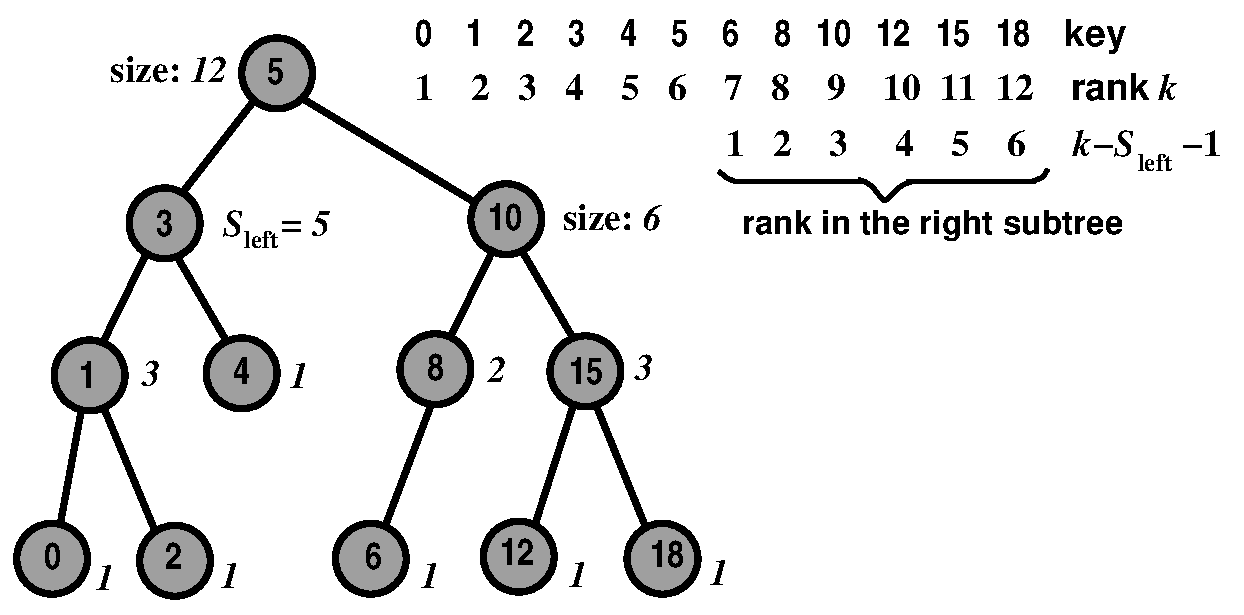
\includegraphics[width=0.6\linewidth]{figs/btr-rank}
%\caption{Binary search tree with rank statistics.}
%\label{btr-rank-sol}
\end{center}
%\end{figure}


\solution{bst-dist}%{ex:3.3.2} 
Under all possible insertion sequences, 
more balanced trees appear more frequently than unbalanced ones. Thus
the balanced trees (and therefore their shapes) displayed below  will 
occur most often.

%\begin{figure}[htbp]
\begin{center}
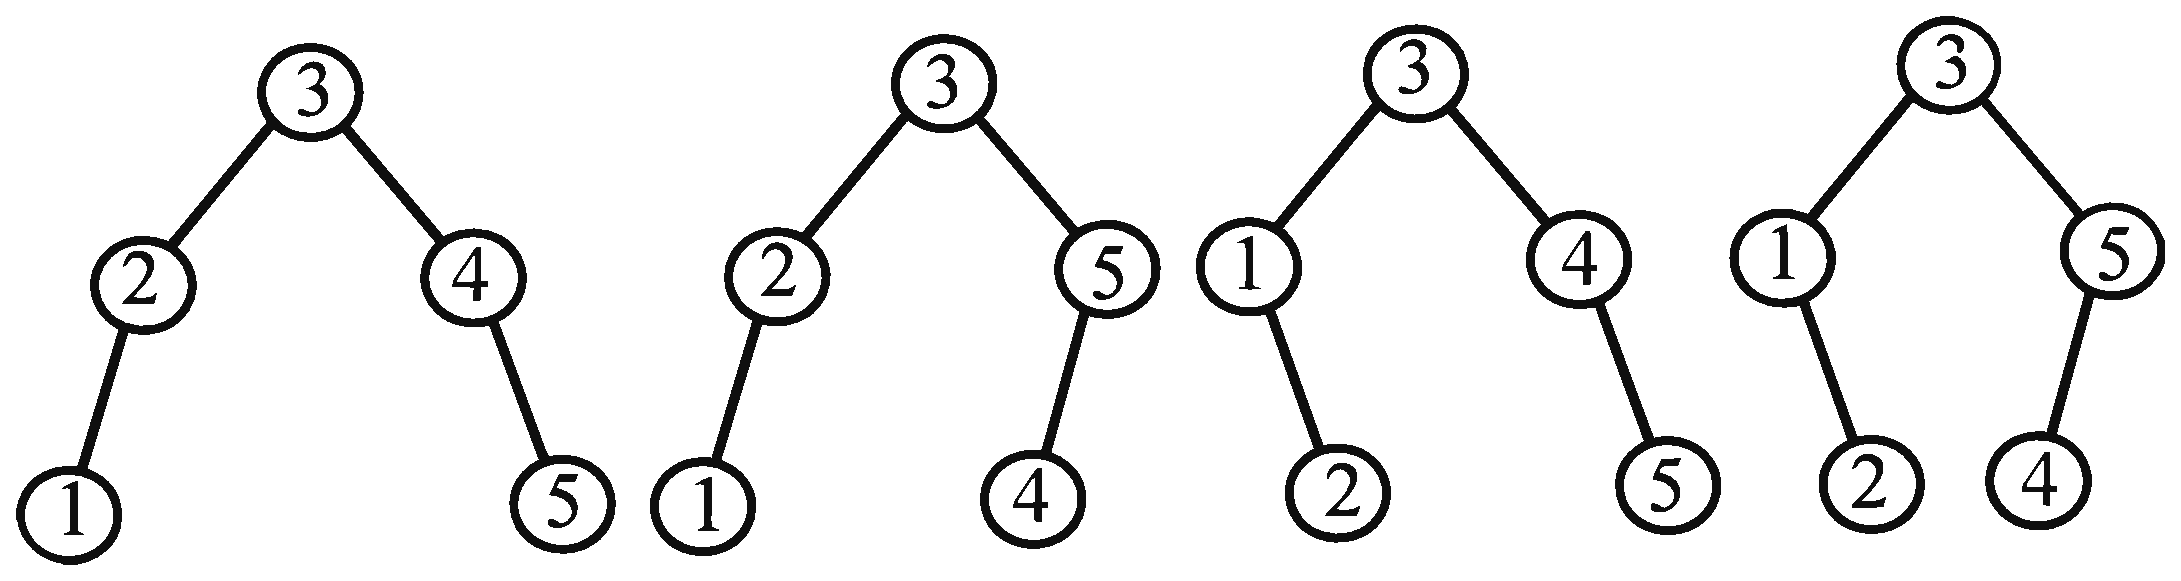
\includegraphics[width=0.65\linewidth]{figs/sol-bst-dist}
%\caption{More frequent balanced BSTs obtained by permutations of $1,2,3,4,5$.}
%\label{fig:sol:bst-dist}
\end{center}
%\end{figure}

\solution{exr:bst-extreme}%{ex:3.3.3}
As was shown in Figure~\ref{btr-4b},
the insertion orders $1423$, $1432$, $1243$, $1234$, $4312$, $4321$,
$4132$, and $4123$ yield a tree of the maximal height 3, while
$2134$, $2143$, $2314$, $2341$, $2413$, $2431$, $3124$, $3142$, $3214$, $3241$, 
$3412$, and $3421$ yield a tree of the minimal height 2.

\solution{exr:bst-sort}%{ex:3.3.4}
Just as in the above solution to Exercise~\ref{exr:bst-min-max-med}, notice 
that according to the ordering relation, the root of a BST behaves like 
the pivot in quicksort because all the keys to its left or to its right 
are smaller or greater, respectively. Therefore, all the keys
can be sorted in ascending order by a recursive tree traversal similar to 
quicksort in that the left subtree is visited first, then the root, then 
the right subtree, so the output of records in order of visiting the nodes 
of the BST yields the ascending order of their keys.  

\solution{exr:redblack:example}%{ex:3.4.1}
Several solutions exist, and two red-black trees with two black nodes
along ``root--leaf'' paths are shown here.
%\begin{figure}[htbp]
\begin{center}
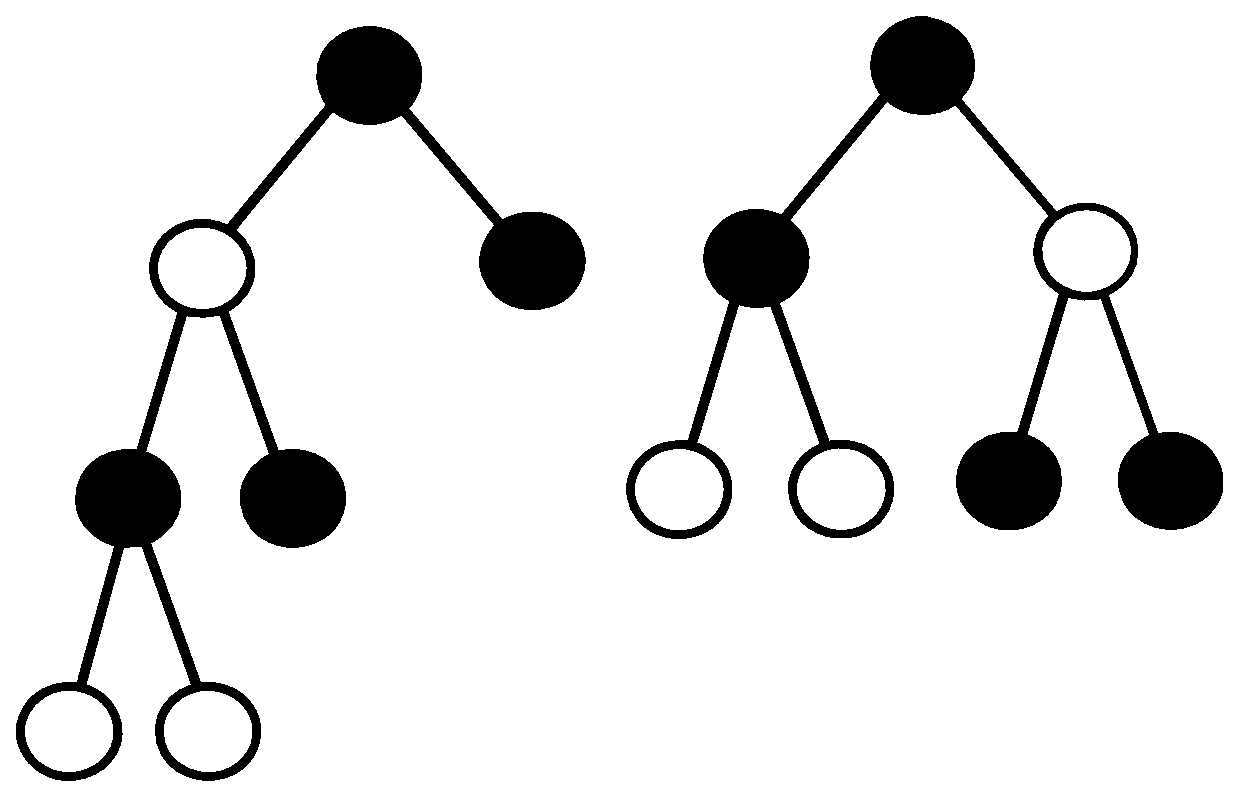
\includegraphics[width=0.35\linewidth]{figs/sol-red-black}
%\caption{Red-black trees with two black nodes along ``root--leaf" paths.}
%\label{fig:sol:red-black}
\end{center}
%\end{figure}

\solution{exr:avl:example}%{ex:3.4.2}
Several solutions exist, and two AVL trees with 7 nodes are shown below
along with the complete binary tree, which is also an AVL tree.
%\begin{figure}[htbp]
\begin{center}
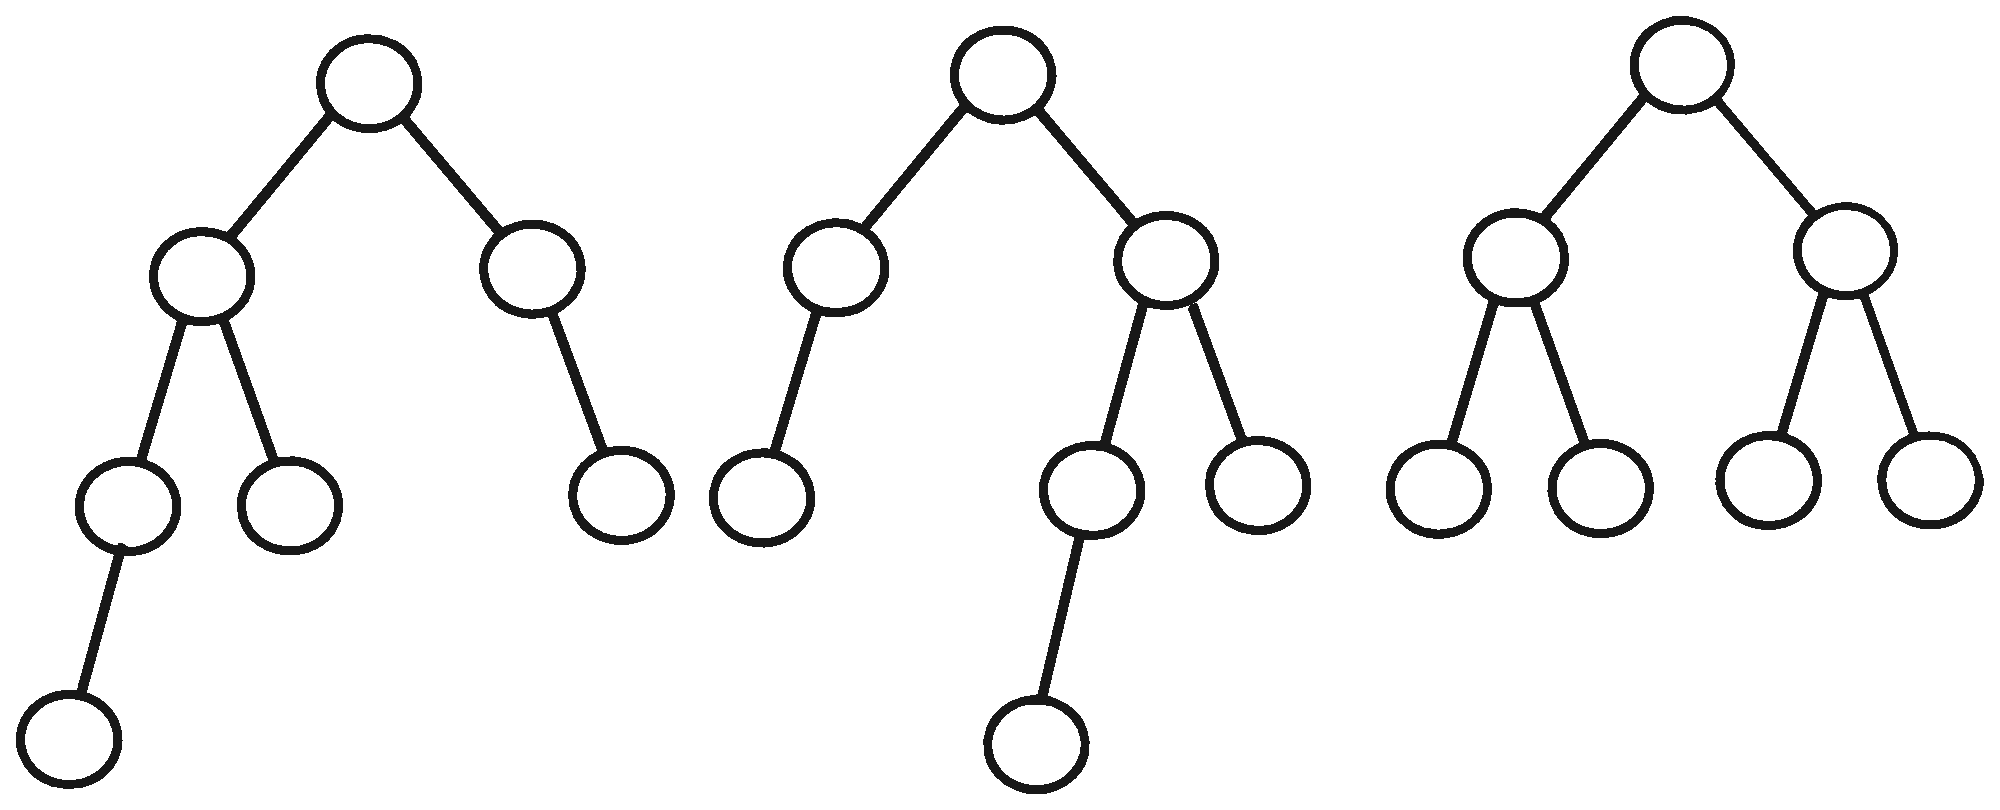
\includegraphics[width=0.5\linewidth]{figs/sol-avl-complete}
%\caption{Two AVL trees with 7 nodes comparing to the complete binary tree.}
%\label{fig:sol:avl}
\end{center}
%\end{figure}

\solution{exr:aa:example}%{ex:3.4.3}
One AA tree with two black nodes along ``root-leaf'' paths, of several
possible solutions, is shown below.
%\begin{figure}[htbp]
\begin{center}
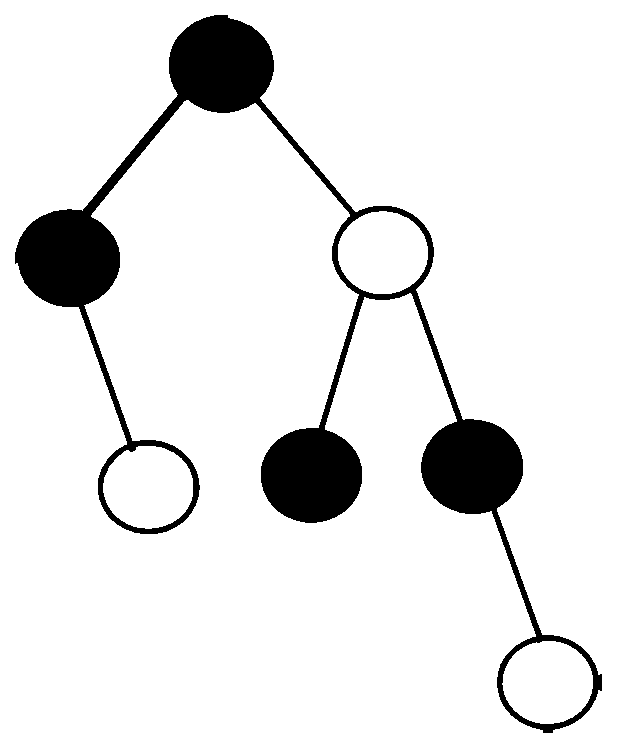
\includegraphics[width=0.15\linewidth]{figs/sol-AA}
%\caption{AA tree with two black nodes along ``root--leaf" paths.}
%\label{fig:sol:AA}
\end{center}
%\end{figure}


\solution{exr:java:hash}%{ex:3.5.1}
For example, 
two strings $s_1 = \mathrm{bC}$ and $s_2 = \mathrm{ab}$ have just the same hash code
$31\times98 + 67 = 31\times97 + 98 = 3105$. Generally, the same hash code is for a 
pair of 2-letter strings, $s_1$ and $s_2$, such that $h(s_1)=h(s_2)$, that is,
$31s_1[0] + s_1[1] = 31s_2[0] + s_2[1]$, or $31(s_1[0] - s_2[0]) = s_2[1] - s_1[1]$.
Let for definiteness, $s_1[0] > s_2[0]$. 
Positive differences between the Unicode values of two capitals (A,B,\ldots,Z) or two small
letters (a,b,\ldots,z) are in the range of $[0..25]$, and between the 
values of a small
and a capital letter are in the range of $[7..57]$. Therefore, only a single pair of
the differences, $s_1[0]-s_2[0] = 1$ and $s_2[1] - s_1[1] = 31$, results in the
same hash codes of two different 2-letter strings. Because there are $25 + 25 = 50$ 
pairs of the first letters such that $s_2[0] = s_1[0]-1$
and 25 pairs of the second letters such that $s_2[1] = s_1[1]+31$, in total $50 \times 25 = 750$ 
pairs out of all possible $52^2 = 2704$ 2-letter strings have the same hash code.

For the even $n$, the hash function is reduced to the weighted sum of
hash codes for the successive 2-letter substrings:
\[
h(s) = 31^{n-2}\left(31s[0]+s[1]\right) +  31^{n-4}\left(31s[2]+s[3]\right) + \ldots + \left(31s[n-2]+s[n-1]\right)
\]
%\newpage
Let $S_m=\{(s_{i:0};s_{i:1}): i=1,\ldots,m\}$ be an arbitrary subset of $m$ different 2-letter pairs 
having each the same hash code $h_i$. Then $2^m$ strings $s$, size of $2m$ letters each, with the
same hash code $h(s)=31^{2m-2}h_0+31^{2m-4}h_1+\ldots+31h_{m-2}+h_{m-1}$ can be built
by concatenating the $m$ substrings, one from each pair:
\(
s = s_{1:\alpha_1}s_{2:\alpha_2}\ldots s_{m:\alpha_m}
\)
providing
$s_{i:0}$ or $s_{i:1}$ are selected in accord with the $i$-th binary digit $\alpha_i$ of
the binary number between 0 and $2^m- 1$. To form $2^{100}$ such strings,
we need to select $m=100$ arbitrary 2-letter pairs, $S_{100}$, having each the same hash code.


%\if 01
%%
\solution{exr:hash:oalp}%{ex:3.5.1}
\begin{center}
{\footnotesize
\begin{tabular}{|l|c|c|c|c|c|c|c|c|c|c|c|c|c|}
\hline
Hash table index& 0& 1& 2& 3& 4& 5& 6& 7& 8& 9& 10& 11& 12 \\
\hline
Insert 10&&&&&&&&&&& \textbf{10}&& \\
\hline
Insert 26& \textbf{26}&&&&&&&&&& 10&& \\
\hline
Insert 52, collision at 0& 26&&&&&&&&&& 10&& \textbf{52} \\
\hline
Insert 76& 26&&&&&&&&&& 10& \textbf{76}& 52 \\
\hline
Insert 13, collision at 0& 26&&&&&&&&& \textbf{13}& 10& 76& 52 \\
\hline
Insert 8& 26&&&&&&&& \textbf{8}& 13& 10& 76& 52 \\
\hline
Insert 3& 26&&& \textbf{3}&&&&& 8& 13& 10& 76& 52 \\
\hline
Insert 33& 26&&& 3&&&& \textbf{33}& 8& 13& 10& 76& 52 \\
\hline
Insert 60, collision at 8& 26&&& 3&&& \textbf{60}& 33& 8& 13& 10& 76& 52 \\
\hline
Insert 42, collision at 3& 26&& \textbf{42}& 3&&& 60& 33& 8& 13& 10& 76& 52 \\
\hline
Resulting hash table& 26&& 42& 3&&& 60& 33& 8& 13& 10& 76& 52 \\
\hline
\end{tabular}
}
\end{center}
%%
%\fi


\solution{exr:hash:oadh}%{ex:3.5.2}
\begin{center}
{\footnotesize
\begin{tabular}{|l|c|c|c|c|c|c|c|c|c|c|c|c|c|}
\hline
Hash table index& 0& 1& 2& 3& 4& 5& 6& 7& 8& 9& 10& 11& 12 \\
\hline
Insert 10&&&&&&&&&&& \textbf{10}&& \\
\hline
Insert 26& \textbf{26}&&&&&&&&&& 10&& \\
\hline
Insert 52, collision at 0, \(\Delta=4\)& 26&&&&&&&&& \textbf{52}& 10&& \\
\hline
Insert 76& 26&&&&&&&&& 52& 10& \textbf{76}& \\
\hline
Insert 13, collision at 0, \(\Delta=1\)& 26&&&&&&&&& 52& 10& 76& \textbf{13}\\
\hline
Insert 8& 26&&&&&&&& \textbf{8}& 52& 10& 76& 13\\
\hline
Insert 3& 26&&& \textbf{3}&&&&& 8& 52& 10& 76& 13\\
\hline
Insert 33& 26&&& 3&&&& \textbf{33}& 8& 52& 10& 76& 13\\
\hline
Insert 60, collision at 8, \(\Delta=4\)& 26&&& 3& \textbf{60}&&& 33& 8& 52& 10& 76& 13\\
\hline
Insert 42, collision at 3, \(\Delta=3\)& 26& \textbf{42}&& 3& 60&&& 33& 8& 52& 10& 76& 13\\
\hline
Resulting hash table& 26& 42&& 3& 60&&& 33& 8& 52& 10& 76& 13\\
\hline
\end{tabular}
}
\end{center}

%\if 01
%%
\solution{exr:hash:sc}%{ex:3.5.3}

\noindent{\footnotesize
\setlength\tabcolsep{5pt}
\begin{tabular}{|l|c|c|c|c|c|c|c|c|c|c|c|c|c|}
\hline
Hash table index& 0& 1& 2& 3& 4& 5& 6& 7& 8& 9& 10& 11& 12 \\
\hline
Insert 10&&&&&&&&&&& \textbf{10}&& \\
\hline
Insert 26& \textbf{26}&&&&&&&&&& 10&& \\
\hline
Insert 52, collision at 0& \{26,\textbf{52}\}&&&&&&&&& & 10&& \\
\hline
Insert 76& \{26,52\}&&&&&&&&& & 10& \textbf{76}& \\
\hline
Insert 13, collision at 0& \{26,52,\textbf{13}\}&&&&&&&&& & 10& 76& \\
\hline
Insert 8& \{26,52,13\}&&&&&&&& \textbf{8}&& 10& 76& \\
\hline
Insert 3& \{26,52,13\}&&& \textbf{3}&&&&& 8&& 10& 76& \\
\hline
Insert 33& \{26,52,13\}&&& 3&&&& \textbf{33}& 8&& 10& 76& \\
\hline
Insert 60, collision at 8& \{26,52,13\}&&& 3&&&& 33& \{8,\textbf{60}\}&& 10& 76& \\
\hline
Insert 42, collision at 3& \{26,52,13\}&&& \{3,\textbf{42}\}&&&& 33& \{8,60\}&& 10& 76& \\
\hline
Resulting hash table& \{26,52,13\}&&& \{3,42\}&&&& 33& \{8,60\}&& 10& 76& \\
\hline
\end{tabular}
}
%%
%\fi

\if 01
\solution{ex:avl:oadh}%{ex:3.6.1}
For an OADH-table, the theoretical estimates for the search 
time are \(T_{ss}(0.75)=1.85\) and \(T_{us}(0.75)=4\) for successful and 
unsuccessful search, respectively. Insertion of a key takes the same time as 
an unsuccessful search, i.e. 4 probes. Deletion of a key takes the 
same time as a successful search, i.e. 1.85 probes.

For an AVL tree, with \(n=1048576=2^{20}\), the search, insertion, and deletion take 
20 steps each. Roughly these steps are equivalent to probes, and it is clear 
from Table 3.5 that since sorting is not a requirement and the hash table                               %%% !!! - ############## Table 3.5
is constructed only once but the other operations are frequent, the OADH-table 
is the best when one only wants to search and remains still the best when one 
wants to insert and delete items frequently.
\fi

%%%%%%%%%%%%%%%%%%%%%%%%%%%%%%%% END AA part %%%%%%%%%%%%%%%%%%%%%%%%%%%

\solution{ex:degree}%{ex:4.1.1} 
Consider a set of arcs \(E\) and
nodes \(V\), we want to construct the digraph \(G=(V,E')\) where
\(E'=E\). We do this by taking the empty digraph \(G'=(V,\{\})\)
and for each arc in \(E\) add it to the graph \(G'\). Each time we
add an arc \((u,v) \in E\) to \(G'\), we are adding one to the
outdegree of node \(u\) and one to the indegree of \(v\). When we
have added all the arcs we get the graph \(G\) and since every time
the outdegree of a node increased, the indegree of a node also
increased. Hence, the sum of the outdegrees equal the sum of the
indegrees.

For a graph, an analogous statement would be that the sum of all
the degrees of all vertices is equal to twice the number
of edges in the graph. This is because each edge contains two 
different vertices.

\solution{ex:distbound}%{ex:4.1.2}
Given that the path exists between nodes \(u\) and \(v\), then there
exists a sequence of nodes \(u,v_1,v_2,\ldots,v_k,v\) such that no node is
repeated. If no node is repeated then \(k \leq n-2\) where \(n\)
is the number of nodes in the digraph. If \(k\) was any greater,
than a node would be repeated, and it would contain a cycle that can be
eliminated.  As \(d(u,v) \leq k+1\), \(d(u,v) \leq n-1\).

\solution{ex:sparse-deg}%{ex:4.1.3}
We have defined sparse being if the number of edges being \(O(n)\)
where \(n\) is the number of nodes. And dense is when the number
of edges are \(\Omega(n^2)\).

The sum of the indegrees of the digraph is
also the number of arcs $m$. The average indegree of
a node is \(\frac{m}{n}\).

For sparse graphs, the number of arcs  $m \in O(n)$, or $m \leq cn$ for
some fixed constant $c$ independent of $n$. Thus, the average indegree is less
than or equal to $c$, which is $O(1)$.

For dense graphs, the number of edges $m \in \Omega(n^2)$, or $m \geq
cn^2$ for some fixed constant $c$ independent of $n$.  Thus, the average 
is greater than or equal to $cn$, which is $\Omega(n)$.

\solution{ex:list2matrix}%{ex:4.2.1}
\[\left[
	\begin{array}{ccccccc}
	0& 0& 1& 0& 0& 0& 0 \\
	1& 0& 0& 0& 0& 0& 0 \\
	1& 1& 0& 0& 0& 0& 0 \\
	0& 0& 0& 0& 1& 1& 1 \\
	0& 0& 0& 0& 0& 1& 0 \\
	0& 0& 0& 1& 1& 0& 1 \\
	0& 1& 1& 0& 0& 0& 0 \\
	\end{array}
\right]\]


\if 11
%%
\solution{ex:matrix2list}%{ex:4.2.2}
\begin{center}
\AdjLists{
$ \begin{array}{l}
7 \\
1~~4~~5 \\
0~~3 \\
0~~6 \\
0~~5 \\
5 \\
\\
5\\
\end{array} $
}
\end{center}
\fi

%\newpage

\solution{ex:listreverse}%{ex:4.2.3}
\[\left[
	\begin{array}{ccccccc}
	0& 1& 1& 0& 0& 0& 0 \\
	0& 0& 1& 0& 0& 0& 1 \\
	1& 0& 0& 0& 0& 0& 1 \\
	0& 0& 0& 0& 0& 1& 0 \\
	0& 0& 0& 1& 0& 1& 0 \\
	0& 0& 0& 1& 1& 0& 0 \\
	0& 0& 0& 1& 0& 1& 0 \\
	\end{array}
\right]\]


\solution{ex:divisible}%{ex:4.2.4}
\(G\):
\[\left[
	\begin{array}{cccccccccccc}
	0& 1& 1& 1& 1& 1& 1& 1& 1& 1& 1& 1 \\
	0& 0& 0& 1& 0& 1& 0& 1& 0& 1& 0& 1 \\
	0& 0& 0& 0& 0& 1& 0& 0& 1& 0& 0& 1 \\
	0& 0& 0& 0& 0& 0& 0& 1& 0& 0& 0& 1 \\
	0& 0& 0& 0& 0& 0& 0& 0& 0& 1& 0& 0 \\
	0& 0& 0& 0& 0& 0& 0& 0& 0& 0& 0& 1 \\
	0& 0& 0& 0& 0& 0& 0& 0& 0& 0& 0& 0 \\
	0& 0& 0& 0& 0& 0& 0& 0& 0& 0& 0& 0 \\
	0& 0& 0& 0& 0& 0& 0& 0& 0& 0& 0& 0 \\
	0& 0& 0& 0& 0& 0& 0& 0& 0& 0& 0& 0 \\
	0& 0& 0& 0& 0& 0& 0& 0& 0& 0& 0& 0 \\
	0& 0& 0& 0& 0& 0& 0& 0& 0& 0& 0& 0 \\
	\end{array}
\right]\]

\(G_r:\)
\[\left[
	\begin{array}{cccccccccccc}
	0&0&0&0&0&0&0&0&0&0&0&0 \\
	1&0&0&0&0&0&0&0&0&0&0&0 \\
	1&0&0&0&0&0&0&0&0&0&0&0 \\
	1&1&0&0&0&0&0&0&0&0&0&0 \\
	1&0&0&0&0&0&0&0&0&0&0&0 \\
	1&1&1&0&0&0&0&0&0&0&0&0 \\
	1&0&0&0&0&0&0&0&0&0&0&0 \\
	1&1&0&1&0&0&0&0&0&0&0&0 \\
	1&0&1&0&0&0&0&0&0&0&0&0 \\
	1&1&0&0&1&0&0&0&0&0&0&0 \\
	1&0&0&0&0&0&0&0&0&0&0&0 \\
	1&1&1&1&0&1&0&0&0&0&0&0 \\
	\end{array}
\right]\]


\if 01
%%
\solution{ex:heaprep}%{ex:4.2.5}
Assuming that arcs only go down the tree (and not up).

Adjacency matrix:
\[\left[
	\begin{array}{ccccccc}
	0& 1& 1& 0& 0& 0& 0 \\
	0& 0& 0& 1& 1& 0& 0 \\
	0& 0& 0& 0& 0& 1& 1 \\
	0& 0& 0& 0& 0& 0& 0 \\
	0& 0& 0& 0& 0& 0& 0 \\
	0& 0& 0& 0& 0& 0& 0 \\
	0& 0& 0& 0& 0& 0& 0 \\
	\end{array}
\right]\]

Adjacency list:
\AdjListx{
\begin{align*}
&7 \\
&1\; 2 \\
&3\; 4 \\
&5\; 6 \\
&\\
&\\
&\\
&\\
&0 \\
\end{align*}
}
%%
\fi


\solution{ex:trav-maze-random}%{ex:5.1.1}
At each time we turn right, else if its a dead end back up as little
as possible. What we are doing is applying to the \emph{visit}
algorithm (Figure~\ref{fig:travcode}) a heuristic, a method of solving 
a problem,    
to the \emph{'choose a grey node \emph{u}'} statement. The \emph{visit}
algorithm allows for any way of choosing which grey node to choose
next, so the way specified in the exercise is a valid way that will,     
eventually, result in finding the exit.

\if 01
%%
\solution{ex:trav-maze-random}%{ex:5.2.1}
This digraph has all 4 type of arcs.

Adjacency list:
\begin{align*}
& 4 \\
& 1,2,3 \\
& 2 \\
& 1 \\
& 2 \\
& 0 \\
\end{align*}
%%
\fi

\solution{ex:DFS-doDFS}%{ex:5.2.2} 
When DFS is run on the graph, the follow timestamps are obtained.

\begin{center}
\begin{tabular}{|c|c|c|c|c|c|c|c|}
\hline
v& 0& 1& 2& 3& 4& 5& 6 \\
\hline
\(seen[v]\)& 0& 2& 1& 6& 7& 8& 9 \\
\hline
\(done[v]\)& 5& 3& 4& 13& 12& 11& 10 \\
\hline
\end{tabular}
\end{center}

Tree arcs:
(0,2),(2,1),(3,4),(4,5),(5,6)

Forward arcs:
(3,5),(3,6)

Back arcs:
(1,0),(2,0),(5,3),(5,4)

Cross arcs:
(6,1),(6,2)


\if 01
%%
\solution{ex:DFS-cross-vs-forward}%{ex:5.2.3}

We have DFS looking at the arc \((u,v)\in E(G)\) at this time, and
want to know if it is a forward arc or a cross arc. A forward arc
is a non-tree arc where \(u\) is an ancestor of \(v\) in the tree
that \(u\) and \(v\) are in. A cross arc is when \(u\) is neither
an ancestor nor descendant of \(v\) in the tree that \(u\) and \(v\)
are in.

We already know that if \(v\) is white it is a tree arc and when
\(v\) is grey it is a back arc. When \(v\) is black it is either a
forward arc, or a cross arc. To determine if its a forward arc,
need to check if \(u\) is an ancestor of \(v\):

\[seen[u] < seen[v] < done[u] < done[v]\]

If this is true then \((u,v)\) is a forward arc, else it is a cross arc.

%%
\fi

\solution{ex:DFS-arc-class}%{ex:5.2.4} 
By using the defintions of these arcs
and also Theorem~\ref{thm:DFS-seen-done}, we can prove each of the three statements.                      

Let \((v,w) \in E(G)\) be an arc. A forward arc is an arc such that
\(v\) is an ancestor of \(w\) in the tree and is not a tree arc.
If the arc \((v,w)\) is in the tree (a tree arc), then \(v\) is
still an ancestor of \(w\). Thus, the arc \((v,w)\) is a tree or
forward arc if and only if \(v\) is an ancestor of \(w\).

By Theorem~\ref{thm:DFS-seen-done}, \(v\) is an ancestor of \(w\) is equivalent to:  

\[seen[v] < seen[w] < done[w] < done[v]\]

The arc \((v,w)\) is a back arc if \(w\) is an ancestor of \(v\)
in the tree and is not a tree arc. If \(w\) is an ancestor of \(v\)
then it cannot be a tree arc by the above proof. This means that
the arc is a back arc if and only if \(w\) is an ancestor of \(v\).

By Theorem~\ref{thm:DFS-seen-done}, \(w\) is an ancestor of \(v\) is equivalent to:

\[seen[w] < seen[v] < done[v] < done[w]\]

The arc \((v,w)\) is a cross arc if neither \(v\) nor \(w\) are the ancestor of the other. 
But, we only need to check if \(w\) is not an ancestor of \(v\). This is because of the order 
that DFS visits these nodes, if it visits \(v\) before \(w\) \((seen[v] < seen[w])\) then 
this will be a tree or forward arc. So to be a cross arc, \(seen[w] < seen[v]\) must be true. 
This means that the arc \((v,w)\) is a cross arc if and only if \(w\) is not an ancestor of \(v\).

By Theorem~\ref{thm:DFS-seen-done}, \(w\) is not an ancestor of \(v\) is equivalent to: 

\[seen[w] < done[w] < seen[v] < done[v]\]


\solution{ex:DFS-timestamps}
(i) Simply apply the rules found in Exercise~\ref{ex:DFS-arc-class},            
the table entries are the type of arc \((u,v)\) would be if the arc existed.

\begin{center}
\begin{tabular}{|c|c|c|c|c|c|c|c|}
\hline
\(u\)& \multicolumn{7}{|c|}{\(v\)} \\
\hline
& 0& 1& 2& 3& 4& 5& 6 \\
\hline
0& & Tree& Forward& Tree& Forward& Forward& Forward \\
\hline
1& Back& & Tree& Cross& Forward& Forward& Forward \\
\hline
2& Back& Back& & Cross& Forward& Tree& Forward \\
\hline
3& Back& Cross& Cross& & Cross& Cross& Cross \\
\hline
4& Back& Back& Back& Cross& & Back& Cross \\
\hline
5& Back& Back& Back& Cross& Tree& & Tree \\
\hline
6& Back& Back& Back& Cross& Cross& Back&  \\
\hline
\end{tabular}
\end{center}

Of course, if some of these arcs existed, and DFS was run on the graph, some of the 
timestamps would change.
\newline 

\noindent
(ii) It would be a back arc.
\newline

\noindent
(iii) No, because they are on different branches of the tree (hence if \((3,2)\) was 
an arc in the graph, it would be a cross arc)
\newline

\noindent
(iv) No, because then when DFS is at time 4, instead of expanding node 4, it would 
expand node 3, and the DFS tree would be entirely different.
\newline 

\noindent
(v) Yes, because it is DFS the tree would be the same (but not if it was BFS), the 
arc would be a forward arc.


\if 01
\solution{ex:DFS-tree-vs-nontree}
At first, looking at the differences between the seen time stamps and the done time 
stamps seems promising. 
If the stamps (either the seen time or the done time) differ by one then its a tree arc. 
But this fails when a node in 
the tree has 3 or more children.

Let \((v,w) \in E(G)\), for this to be a tree arc \(v\) must be an
ancestor of \(w\) and there is no node \(u\) in between \(v\) and
\(w\) in the tree. Let \(A(u_1,u_2)\) be true if \(u_1\) is a
ancestor of \(u_2\) for any two nodes in \(E(G)\): \[(v,w) \in E(G)
\text{ is a tree arc} \iff A(v,w), \forall u \in E(G), \neg A(v,u)
\wedge \neg A(u,w), u \neq v,w \]

Thus, because \(A(u_1,u_2)\) is computable with only the timestamps
(Theorem~\ref{thm:DFS-seen-done}), there is a way to distinguish tree arcs from non-tree
arcs just by looking at the timestamps.
\fi

\if 01
%%
\solution{ex:DFS-graph-no-cross}%{ex:5.2.7}
Let \((u,v) \in E(G)\), for this to be a cross edge, when node \(u\) is being examined by DFS, node \(v\) has to have 
been done. Except, when node \(v\) is being examined, one of its
neighbours is node \(u\) and so node \(v\) will never 
be done before node \(u\) is done. Therefore, there are no cross edges on a DFS tree on a graph \(G\).

\solution{ex:DFS-false-conj}%{ex:5.2.8}
Adjacency list:
\begin{align*}
& 3 \\
& 1,2 \\
& 0 \\
& \\
& 0 \\
\end{align*}

If \(v=1\) and \(w=2\) then even though \(w\) is reachable from
\(v\), it is not a descendant of \(v\).  This is because the path
passes through both their ancestors. Thus, the conjecture would be
true if instead of \(w\) being a descendant of \(v\) that the two
nodes share a common ancestor (i.e.: in the same DFS tree).

%%
\fi

\solution{ex:DFS-prepostorder}%{ex:5.2.9} 
The order of the nodes in the digraph in the \(seen\) array is equal to the preorder labeling 
of the nodes, and the order of the nodes in the diagraph in the \(done\) array is equal to the 
post order labeling of the nodes.


\solution{ex:white-path}%{ex:5.2.10}
To prove via induction, we need both a base case and an inductive step.

The base case is when there are no white nodes as neighbours of node \(s\), then the 
algorithm does no recursion and returns. In this case
\texttt{recursiveDFSvisit} only visits node \(s\), which is intended.

The inductive step is that given all the white nodes that are
neighbours of node \(s\) 
our theorem is true for them, then it is also true for node \(s\). 
For each node reachable from \(s\) 
via a path of white nodes, the start of every path is one of the
neighbours of \(s\). Because the 
call to \texttt{recursiveDFSvisit} with input \(s\) only terminates when the 
recursive calls with input of each of the white
neighbours of \(s\) finish. 
All the recursive calls then cover each of the paths from \(s\) to 
each node reachable by a path of white nodes, and thus satisfies the 
inductive step.

Finally, because each path cannot have a loop in it, there is 
a finite number of 
recursions and \texttt{recursiveDFSvisit} is guaranteed to terminate.

Therefore, by mathematical induction, Theorem~\ref{thm:white-path} is true.

\if 01
\solution{ex:doBFS}%{ex:5.3.1}
\begin{center}
\begin{tabular}{|c|c|c|c|c|}
\hline
Queue indices& 0& 1& 2& 3 \\
\hline
Adding node 0& 0& & & \\
\hline
Adding node 2& 0& 2& & \\
\hline
Deleting node 0& 2& & & \\
\hline
Adding node 1& 2& 1& & \\
\hline
Deleting node 2& 1& & & \\
\hline
Deleting node 1& & & & \\
\hline
Adding node 3& 3& & & \\
\hline
Adding node 4& 3& 4& & \\
\hline
Adding node 5& 3& 4& 5& \\
\hline
Adding node 6& 3& 4& 5& 6 \\
\hline
Deleting node 3& 4& 5& 6 & \\
\hline
Deleting node 4& 5& 6 & & \\
\hline
Deleting node 5& 6 & & & \\
\hline
Deleting node 6& & & & \\
\hline
\end{tabular}
\end{center}

The resulting BFS forest is given below:

Adjacency list:
\begin{align*}
&7 \\
&2 \\
& \\
&1 \\
&4,5,6 \\
& \\
& \\
& \\
&0 \\
\end{align*}

%%%%
\solution{ex:BFS-back-vs-cross}%{ex:5.3.2}
Simply use Theorem~\ref{thm:BFS-arcclass}.


\solution{ex:DAG-vs-tree}%{ex:5.5.1}
Adjacency list:
\begin{align*}
&2 \\
&1 \\
&0 \\
&0 \\
\end{align*}
%%%%
\fi


\solution{ex:DAG-sink}%{ex:5.5.2}
By Theorem~\ref{thm:topDAG}, every DAG has a topological ordering \((v_1,v_2,...v_n)\) such that 
there are no arcs \((v_i,v_j) \in E(G)\) such that \(i < j\). This means that there are no arcs 
going from right to left in the topological ordering. This means that node \(v_1\) has no 
arcs going into it and node \(v_n\) has no nodes going away from it, they are respectively, 
a source and sink node. Therefore for every DAG there is at least one source and sink node.


\if 01
%%
\solution{ex:sillytopsort}%{ex:5.5.3}
In the following example, using the visiting times when running DFS on it results in the sink 
being in the middle of the topological ordering:

Adjacency list:
\begin{align*}
&3 \\
&1,2 \\
& \\
&1 \\
&0 \\
\end{align*}

Therefore, in general, the visiting time is not a topological ordering.
\fi

\solution{ex:profP}%{ex:5.5.4}
Shirt, hat, tie, jacket, glasses, underwear, trousers, socks, shoes, belt.


\solution{ex:zero-indeg-runtime}%{ex:5.5.5}
The standard implementation uses an array of indegrees.  This can
be computed in time $O(m)$ from either adjacency lists or adjacency
matrices.  The algorithm can find a node $v$ of degree $0$ in time 
$O(n)$ and can decrement the indegrees of the neighbours of $v$
in constant time for adjacency lists.  Since we have at most $m$ decrements 
of elements of the array of indegree, the running
time is at most $O(n^2+m)$.  If a priority queue is used to 
extract nodes of indegree 0 the running time slightly improves.

\solution{ex:forest}%{ex:5.5.6}
Simply delete vertices with 0 or 1 edges on them from the graph (including the edges), 
if at anytime there are no vertices with the number of edges less than 2, then the graph 
has a cycle. Otherwise, if the entire graph can be deleted by only deleting vertices with 
0 or 1 edges, then the graph is acyclic.

%\newpage

\solution{ex:DFSfails}%{ex:5.6.1} 

\begin{tabular}{ll}
\begin{minipage}[b]{3cm}
Adjacency list:\\
\AdjLists{
$\begin{array}{l}
4 \\
1, 2 \\
0 \\
3 \\
2 \\
\end{array} $
}\\
\end{minipage}
& \raisebox{-.5cm}{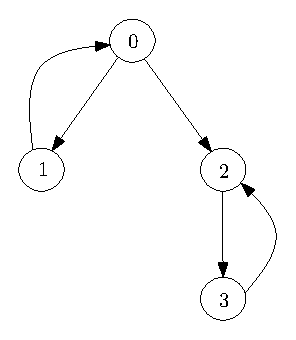
\includegraphics[width=3cm]{figs/dfstopofail}}
\end{tabular}

There are two strongly connected components in this graph, 
DFS only finds one tree.


\if 01
%%
\solution{ex:dolinscc}%{ex:5.6.2}
Need to first run BFS on the digraph \(G\) in Example 5.20 getting the               %%% !!! - ############## Example 5.20 \label{eg:scc}
resulting forest F. Then run DFS on the reverse digraph \(G_r\) choosing 
each root from among the white nodes that finished latest in the resulting 
forest F. Then each DFS tree in the search of \(G_r\) contains one of the 
strong components.

Reverse ordering of nodes by finish time running DFS on \(G\): \{4,5,0,3,2,1\}

Resulting forest running DFS on \(G_r\) choosing new roots in the 
order given above:

Adjacency list:
\begin{align*}
&6 \\
&2 \\
& \\
&3 \\
& \\
&5 \\
& \\
\end{align*}

So there are three strong components: \{4,5\},\{0,2,3\},\{1\}.

%%
\fi

\solution{ex:shortest-cycle-thm}%{ex:5.7.1}

\begin{tabular}{ll}
\begin{minipage}[b]{3cm}
Adjacency list:\\
\AdjLists{
$\begin{array}{l}
5 \\
1, 2, 3 \\
0, 4 \\
0, 4 \\
0, 2 \\
\end{array} $
}\\
\end{minipage}
& \raisebox{-.5cm}{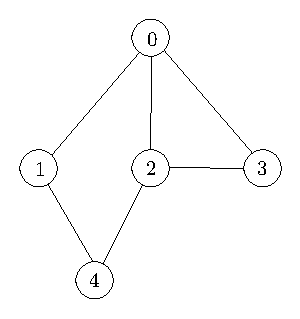
\includegraphics[width=3cm]{figs/bfscyclefail}}
\end{tabular}

If the algorithm does not check to the end of the level, it will return that the 
shortest cycle is \{0,1,4,2\} instead of \{0,2,4\}.

\if 01
%%
\solution{ex:shortest-cycle-runtime}%{ex:5.7.2}
The worst case time complexity of the algorithm is \(O(n+e)\), as it only needs to 
run \texttt{dfsvisit} on each node once, which then does constant number of 
operations on each of its edges. 
%%
\fi

\solution{ex:do2col}%{ex:5.7.3}
We need to find two disjoint subsets. Consider the number of 1's (it can just as 
easily be the number of 0's) to be \(k\) in a bit vector of length \(n\), an edge can only 
be between another bit vector with either \(k-1\) or \(k+1\) 1's. This is because if the 
number of 1's is less than \(k-1\) or greater than \(k+1\) then there will be more 
than 1 difference in the bits. Also, two different bit vectors with the same number 
of 1's will not have an edge because they will differ in two places exactly 
(not the required one).

One way of satisfying this condition is if all the odd number of 1's are on one side, 
and all the even number of 1's are on the other. This means that for any \(n\)-cube you 
can find a bipartite consisting of the odd number of 1's bit vectors in one group, 
and the even number of 1's in the other.

\solution{ex:radius}
The running time is the same as the time to compute the distance matrix.
The eccentricity of a node $v$ is simply the maximum
entry of row $v$ of the distance matrix.  The radius is the
minimum over all maximum values per row.  This can be computed in time $\Theta(n^2)$
if we have access to a distance matrix.

\solution{ex:SSSP-neg-cycle}
If a cycle $v_1,v_2,\ldots,v_k$ exists with the sum of its arc weights is less than zero 
then we can find a walk of total weight as small as we want from $v_1$ to $v_2$ by repeating
the cycle as many times as we want before stopping at $v_2$.

\solution{ex:dijk-proof}
Property P2 fails if we allow arcs of negative weight.  Suppose $u$ is the next
vertex added to $S$.  If arc $(u,w)$ is of negative weight for some other vertex $w$
that is currently in $S$, then the previous distance from $s$ to $w$, $dist[w]$, may no 
longer be the smallest.

%\newpage
\solution{ex:floyd-neg-cycle}
If a diagonal entry in the distance matrix ever becomes less than zero when
using Floyd's algorithm then know that a negative weight cycle has been found.

\solution{ex:doMST}
For this weighted graph, both Prim's and Kruskal's algorithms will find the 
unique minimum spanning tree of weight $9$.
%, which corresponds to the Hamiltonian path $0,2,4,5,3,1$


%% \if 01 % part 3 solutions
%% 
%% \solution{ex:A2}
%% \centerline{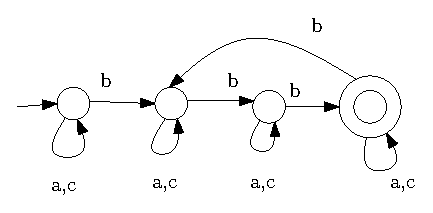
\includegraphics[width=3.2in]{figs/automata3k_b}}
%% 
%% \solution{ex:A4}
%% %\begin{proof}
%% Assume a DFA machine $M$ with $m$ states accepts $L=\{0^n1^{2n}
%% \mid n \geq 0\}$.  Consider what states the machine $M$ reaches with
%% each of the following strings $x_1=0$, $x_2=00$, \ldots, $x_m=0^m$,
%% $x_{m+1}=0^{m+1}$.  Since $M$ has only $m$ states there must be
%% two strings $x_i$ and $x_j$ ($i\not=j$) that reach the same state.
%% Now consider the two strings $0^i1^{2i}$ and $0^j1^{2i}$.  The machine
%% $M$ must accept both (or neither).  Thus $M$ does not accept $L$.
%% The same argument holds for any finite state machine.
%% %\end{proof}
%% 
%% \if 11
%% \solution{ex:Aprime}
%% Since there are an infinite number of prime numbers, any DFA that
%% accepts this language must have at least one cycle formed by transitions
%% via the character 0.  Let $k$ be the length of one such reachable cycle.
%% Let $x$ be a string that lands on an accepting state on this cycle 
%% (that is, $x$ has a prime number of 0's).  Any string $x0^k$ is also accepted 
%% by the DFA.  This shows that the number of primes less than $n$, as $n$ 
%% approaches $\infty$, is $\Omega(n/k)$.  This contradicts the Prime Number 
%% Theorem: The number of primes less then $n$, $\Theta(n)$, is proportional 
%% to $n/\ln(n)$. 
%%  [that is, $\lim_{n \rightarrow \infty } \Theta(n) / (n/ln(n)) = 1$ ]
%% \fi
%% 
%% 
%% 
%% \solution{ex:A5}
%% There are two common ways to build an automaton for the
%% intersection of
%% two regular languages $L_1$ and $L_2$ that are accepted by DFA $M_1$ and
%% $M_2$, respectively.
%% 
%% Method 1: Build a new automaton $M$, where the states $Q$ are $Q_1
%% \times Q_2$.  Accepting states $(q_1,q_2) \in Q$ if and only if
%% $q_1$ and $q_2$ are accepting states of $M_1$ and $M_2$. Transitions
%% $\delta((q_1,q_2),c)=(q'_1,q'_2)$ if and only if $\delta_1(q_1,c)=q'_1$
%% and $\delta_2(q_2,c)=q'_2$. The unique starting state is $(s_1,s_2)$
%% where $s_1$ and $s_2$ are the start states for $M_1$ and $M_2$,
%% respectively.
%% 
%% Method 2: Use set theory fact that $L_1 \cap L_2 =
%% \overline{\overline{L_1} \cup \overline{L_2}}$, where $\overline{L} =
%% \Sigma^* \setminus L$.  We construct an automaton $M'$ for
%% $\overline{L}$ by taking a DFA $M$ for $L$ and changing accept
%% states to non-accept states (and non-accept states to accept states).
%% 
%% \if 01
%% %%
%% \solution{ex:diff}
%% First note that $L_2 \setminus L_1 = L_2 \cap \overline{L_1} =
%% \overline{\overline{L_2} \cup L_1}$.  Then do the following. \\
%% 1. Build DFA $M_3$ for $\overline{L_2}$.  (swap accept/reject states) \\
%% 2. Build NFA $M_4$ for $\overline{L_2} \cup L_1$.  \\
%% 3. Convert $M_4$ to DFA $M_5$.\\
%% 4. Build DFA $M$ from $M_5$. (swap accept/reject states)
%% %%
%% \fi
%% 
%% \solution{ex:even}
%% Use something like: $0\mid1(0\mid1){}^*0$
%% 
%% \solution{ex:RE}
%% One possible regular expression would be $(a|b|\epsilon)b(ab)^*(b|\epsilon)$.
%% 
%% %\newpage
%% \solution{ex:nfaclosure}
%% One possible answer is:\\
%% \centerline{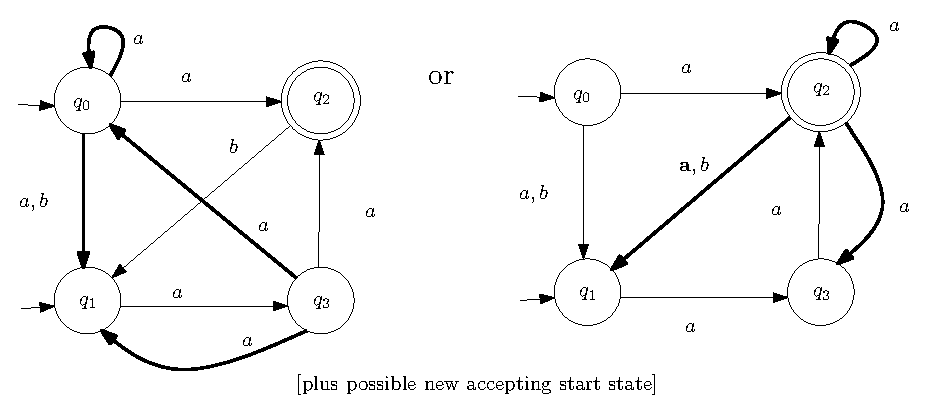
\includegraphics[width=4.2in]{figs/NFAforClosureAns}}
%% 
%% 
%% \begin{samepage}
%% \solution{ex:nfaconcat}
%% Two possible solutions are:\\
%% \centerline{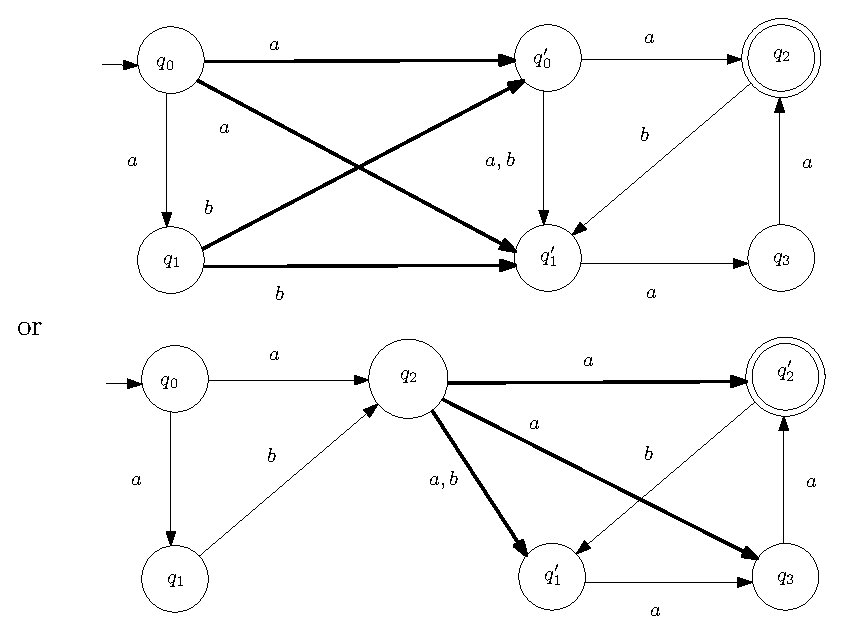
\includegraphics[width=4.0in]{figs/NFAforConcatAns}}
%% \end{samepage}
%% 
%% \solution{ex:A3}
%% \def\inclans{1}
%% Minimum length distinguishers for several pairs of states $s_1$ and $s_2$ 
%% are given in the following table.\\
%% \begin{minipage}{\textwidth}
%% \setlength\tabcolsep{16pt}
%% \setlength\arrayrulewidth{.5pt}
%% %\renewcommand{\baselinestretch}{1.5}\large\normalsize
%%         \begin{tabular}{|c|c|c|}
%%         \hline
%%         State $s_1$ & State $s_2$ & \hspace*{2cm} Distinguisher
%% \hspace*{2cm}  \\   \hline
%%         0 & 1 & \ifnum\inclans=1{$a$} (or $b$)\fi \\
%%         \hline
%%         0 & 5 & \ifnum\inclans=1{$aa$} (or others of length 2)\fi \\
%%         \hline
%%         1 & 2 & \ifnum\inclans=1{N/A}\fi \\
%%         \hline
%%         1 & 3 & \ifnum\inclans=1{$\epsilon$}\fi \\
%%         \hline
%%         3 & 4 & \ifnum\inclans=1{$a$} (or $b$)\fi \\
%%         \hline
%%         \end{tabular}
%% \end{minipage}
%% 
%% \solution{ex:naive}
%% Let $X$=aab and $Y$=aaaaaaa.
%% 
%% \solution{ex:autsizesearch}
%% We observe that each pair of prefix states has a distinguisher.
%% For states $q_i$ and $q_j$, $i<j$, consider the suffix $X[j+1,\ldots,m-1]$.
%% 
%% %\newpage
%% 
%% \solution{ex:computeNext}
%% First note that \verb|next|[$i$] $< i$ and $j+1 \leq i$ at
%% all times in the function \algfont{computeNext}.  At the start of 
%% each \textbf{while} iteration, consider the change to 
%% the state of the variables $i$ or $j$.  Either the value of $i$ increases or 
%% the value of $i-j$ increases (and
%% neither of these values decrease).  Since the function terminates when $i$
%% reaches $m$ the value of $i-j$ can also increase at most $m$ times; this is because
%% $i-j-1$ is a lower bound for $i$.  Thus, there are at most $2m$ iterations of
%% the \textbf{while} loop, which shows the algorithm runs in $O(m)$ time.
%% 
%% \newcommand{\M}{\hspace*{1in} (*)}
%% 
%% \solution{ex:G0}
%% \begin{eqnarray*}
%%   \X{E}  & \rightarrow & \X{E} + \X{T} \:|\:\X{E} - \X{T}\:|\:\X{T} \\
%%   \X{T}  & \rightarrow & \X{T} * \X{F} \:|\:\X{T} / \X{F}\:|\:\X{F} \\
%%  \X{F}  & \rightarrow & \X{F} \verb|^| \X{P}  \:|\: \X{P} \M \\
%%  \X{P}  & \rightarrow & ( \:\X{E}\: ) \:|\: \X{N} \hspace{8pt}\M \\
%%   \X{N}  & \rightarrow & \X{N} \X{D}\:|\: \X{D} \\
%%   \X{D}  & \rightarrow & \mbox{0} \:|\: \mbox{1}\:|\: \mbox{2}\:|\: \mbox{3}\:|\: \mbox{4}\:|\: \mbox{5}\:|\: \mbox{6}\:|\: \mbox{7}\:|\: \mbox{8}\:|\: \mbox{9}
%% \end{eqnarray*}
%% 
%% \solution{ex:G1}
%% With `.' denoting any character except newline `\verb|\n|' and
%% `\verb|\*|' being an escaped '*' we can use the following regular
%% expression.
%% \begin{verbatim}
%%      ('\n' | '\t' | ' ' | //.*\n | /\*(.|'\n')*\*/)+
%% \end{verbatim}
%% 
%% \solution{ex:G2}
%% \begin{enumerate}
%% \item $\ \X{L_1} \;\, \rightarrow \;\, \epsilon \mid  00\X{L_1}11 $
%% \item $
%% \begin{array}{ccl}
%%   \X{L_2}  & \rightarrow & \X{M} \mid 0\X{L_2}1 \\
%%   \X{M}  & \rightarrow & 1 \mid \X{M}1 \\
%% \end{array} $
%% \end{enumerate}
%% 
%% \solution{ex:G3}
%% \begin{enumerate}
%% \item $
%% \begin{array}{ccl}
%%   \X{E_1}  & \rightarrow & aa \mid \X{B} \mid cc \\
%%   \X{B}  & \rightarrow & \epsilon \mid \X{B}b \\
%% \end{array} $
%% \item $
%% \begin{array}{ccl}
%%   \X{E_2}  & \rightarrow & \X{T_1}aa \mid \X{T_2} \\
%%   \X{T_1}  & \rightarrow & \epsilon \mid a\X{T_1} \mid b\X{T_1} \\
%%   \X{T_2}  & \rightarrow & \epsilon \mid bbaa\X{T_2} \\
%% \end{array} $
%% \end{enumerate}
%% 
%% \solution{ex:G4}
%% $$a^+(bc)^+c^+$$
%% 
%% \solution{ex:G5}
%% \begin{eqnarray*}
%%   \X{L}  & \rightarrow & \X{F}\X{G} \\
%%   \X{F}  & \rightarrow & \epsilon \\
%%   \X{G}  & \rightarrow & \X{D_0}\X{G}0 \mid \X{D_1}\X{G}1 \mid \X{E} \\
%%   \X{F}\X{D_0} & \rightarrow & \X{F}0 \\
%%   \X{F}\X{D_1} & \rightarrow & \X{F}1 \\
%%   1\X{D_0}  & \rightarrow & \X{D_0}1 \\
%%   1\X{D_1}  & \rightarrow & \X{D_1}1 \\
%%   0\X{D_0}  & \rightarrow & \X{D_0}0 \\
%%   0\X{D_1}  & \rightarrow & \X{D_1}0 \\
%%   \X{E}  & \rightarrow & \X{D_0}\X{E} \mid \X{D_1}\X{E} \mid 1\X{E} \mid
%% 0\X{E} \mid \# \\
%% \end{eqnarray*}
%% 
%% \fi  % part 3
